\documentclass[a4paper,10pt, fleqn]{article}
\usepackage{graphicx} %Paquete para ingresar gráficos.
\usepackage{hyperref}
\usepackage{fancybox}
\usepackage[utf8]{inputenc}
\usepackage{placeins}
\usepackage{float}
\usepackage{caption}
\usepackage{multirow}


\usepackage{fancyhdr}
\pagestyle{fancy}
\fancyhf{}

\setlength{\headheight}{22.55pt}

\renewcommand{\footrulewidth}{0.4pt}
\renewcommand{\headrulewidth}{0.4pt}

\fancyhead[L]{{\textsf{Facultad de Ingeniería de la Universidad de Buenos Aires \\ 75.43 Introducción a los Sistemas Distribuidos}}}

\fancyhead[R]{\thepage}
\fancyfoot[L]{
	{\textsf{Trabajo Práctico Grupal: Diseño y configuración sobre una topología de red.}} \\
	{\textsf{Integrantes: Díaz Ortiz, Durán, Linardos, Stamato, Tamiozzo, Torres Feyuk.}}
}
		

\title{ \author{}
\setlength{\unitlength}{1cm}
\thispagestyle{empty}

\begin{picture}(10,0)
  \put(0,0){
\includegraphics[width=1.5cm, height=3cm]{Portada/Logo1.png}}
  \put(10.5,0){
\includegraphics[width=3cm, height=3cm]{Portada/Logo2.png}}
\end{picture}
\\[1.5cm]

\begin{center}
	\textbf{{\Huge Facultad de Ingeniería \\ Universidad de Buenos Aires}}\\[2cm]
	{ 75.43 Introducción a los Sistemas Distribuidos.}\\[0.5cm]
	{ Trabajo Práctico Grupal: Diseño y configuración sobre una topología de red.}\\[2.5cm]
\end{center}

\begin{table}[!htbp]
	\textbf{Integrantes:} \\[0.5cm]

 	\begin{tabular}{|l|l|l|}
		\hline
		\textbf{Padrón} & \textbf{Nombre} & \textbf {Email} \\
		\hline
		89775 & Díaz Ortiz, Ramiro &ramiro.do@gmail.com \\
		\hline
		89575 & Durán, Adrián  & adrianmdu@gmail.com \\
		\hline
		89567 & Linardos, Leandro &leandro.linardos@gmail.com \\
		\hline
		91018 & Stamato, Alejandra &alejandra.stamato@gmail.com \\
		\hline
		90746 & Tamiozzo, Ayelén Sol & ayelenst@gmail.com \\
		\hline
		89579 & Torres Feyuk, Ezequiel & ezequiel.torresfeyuk@gmail.com \\
		\hline	
	\end{tabular}
\end{table}

\date{}
 }

\begin{document}
\maketitle 

\tableofcontents 
\newpage

\section{Determinación de subredes}
A partir de la topología entregada y el espacio de direccionamiento asignado, se procedió a realizar el \textit{subnetting} de la red. El espacio 
de direccionamiento asignado es el mostrado en la tabla \ref{tab001}. La resolución de direcciones asignadas que se realizó siguiendo el estandar
esbozado en el \textit{RFC 950} se muestra en la tabla \ref{tab002}. La determinación de las redes y el nombre asociado a cada una se muestra en 
la figura \ref{fig001}. \\

\begin{table}[!htpb]
	\centering
	\begin{tabular}{|c|c|c|c|c|}
		\hline
		Tipo de Red & Dirección de Red & Máscara de Red & Red Privada & Detalles \\
		\hline
		C & 192.168.25.0 & 255.255.255.0 & Si & - \\
		\hline
		A & 10.111.25.0 & 255.255.255.0 & Si & - \\
		\hline
		B & 157.63.5.0 & 255.255.255.0 & No & Internet \\
		\hline
		A & 10.7.5.64 & 255.255.255.192 & Si & Frame Relay \\
		\hline
		A & 10.61.5.0 & 255.255.255.0 & Si & - \\
		\hline
		A & 10.61.6.128 & 255.255.255.128 & Si & - \\
		\hline
		A & 10.61.7.128 & 255.255.255.128 & Si & - \\
		\hline
	\end{tabular}
	\caption{Redes asignadas}
	\label{tab001}
\end{table}
		
\begin{table}[!htbp]
  \begin{tabular}{|c|c|c|c|c|c|c|}
    \hline
	Nombre & Incluye & \#Host & \#Routers & Total & Bloque & Dirección de red \\ \hline
	Amapola & Web Server & 240 & 4 & 244 & 256 & 192.168.25.0/24 \\ \hline
	Begonia & ~ & 29 & 3 & 32 & 64 & 10.111.25.192/26 \\ \hline
	Clavel & Telnet Server & 250 & 2 & 252 & 256 & 10.61.5.0/24 \\ \hline
	Dalia & ~ & 16 & 2 & 18 & 32 & 10.111.25.128/27 \\ \hline
	Espuela & Telnet Server & 17 & 3 & 20 & 32 & 10.61.6.128/27 \\ \hline
	Fresia & ~ & 9 & 4 & 13 & 16 & 10.111.25.160/28 \\ \hline
	Geranio & FTP Server & 124 & 1 & 125 & 128 & 10.111.25.0/25 \\ \hline
	Hortensia & ~ & 120 & 4 & 124 & 128 & 10.61.7.128/25 \\ \hline
	Iris & ~ & 8 & 2 & 10 & 16 & 10.111.25.176/28 \\ \hline
	Jazmín & ~ & 7 & 1 & 8 & 16 & 10.61.6.160/28 \\ \hline
	Kentia & Internet & 0 & 2 & 2 & 4 & 157.63.5.0/30 \\ \hline
	Lirio & ~ & 24 & 3 & 27 & 32 & 10.61.6.192/27 \\ \hline
	Margarita & PPP & 0 & 2 & 2 & 4 & 10.61.6.176/30 \\ \hline
	Narciso & PPP & 0 & 2 & 2 & 4 & 10.61.6.180/30 \\ \hline
	Orquídea & FR – R1/R8 & 0 & 2 & 2 & 4 & 10.7.5.64/30 \\ \hline
	Petunia & FR – R1/R9 & 0 & 2 & 2 & 4 & 10.7.5.68/30 \\ \hline
	Quimonant & FR – R1/R15 & 0 & 2 & 2 & 4 & 10.7.5.72/30 \\ \hline
	Rosa & FR – R8/R9 & 0 & 2 & 2 & 4 & 10.7.5.76/30 \\ \hline
	Siempreviva & FR – R8/R15 & 0 & 2 & 2 & 4 & 10.7.5.80/30 \\ \hline
	Tulipán & FR – R9/R15 & 0 & 2 & 2 & 4 & 10.7.5.84/30 \\ \hline
	Ulmaria & Internet & 0 & 2 & 2 & 4 & 157.63.5.4/30 \\ \hline
	Violeta & Tunnel & 0 & 2 & 2 & 4 & 10.61.6.184/30 \\	
    \hline
  \end{tabular}
  \captionof{table}{Tabla de asignación de redes}
	\label{tab002}
\end{table}

\begin{figure}[!htpb]
      \centering
      \begin{center}
      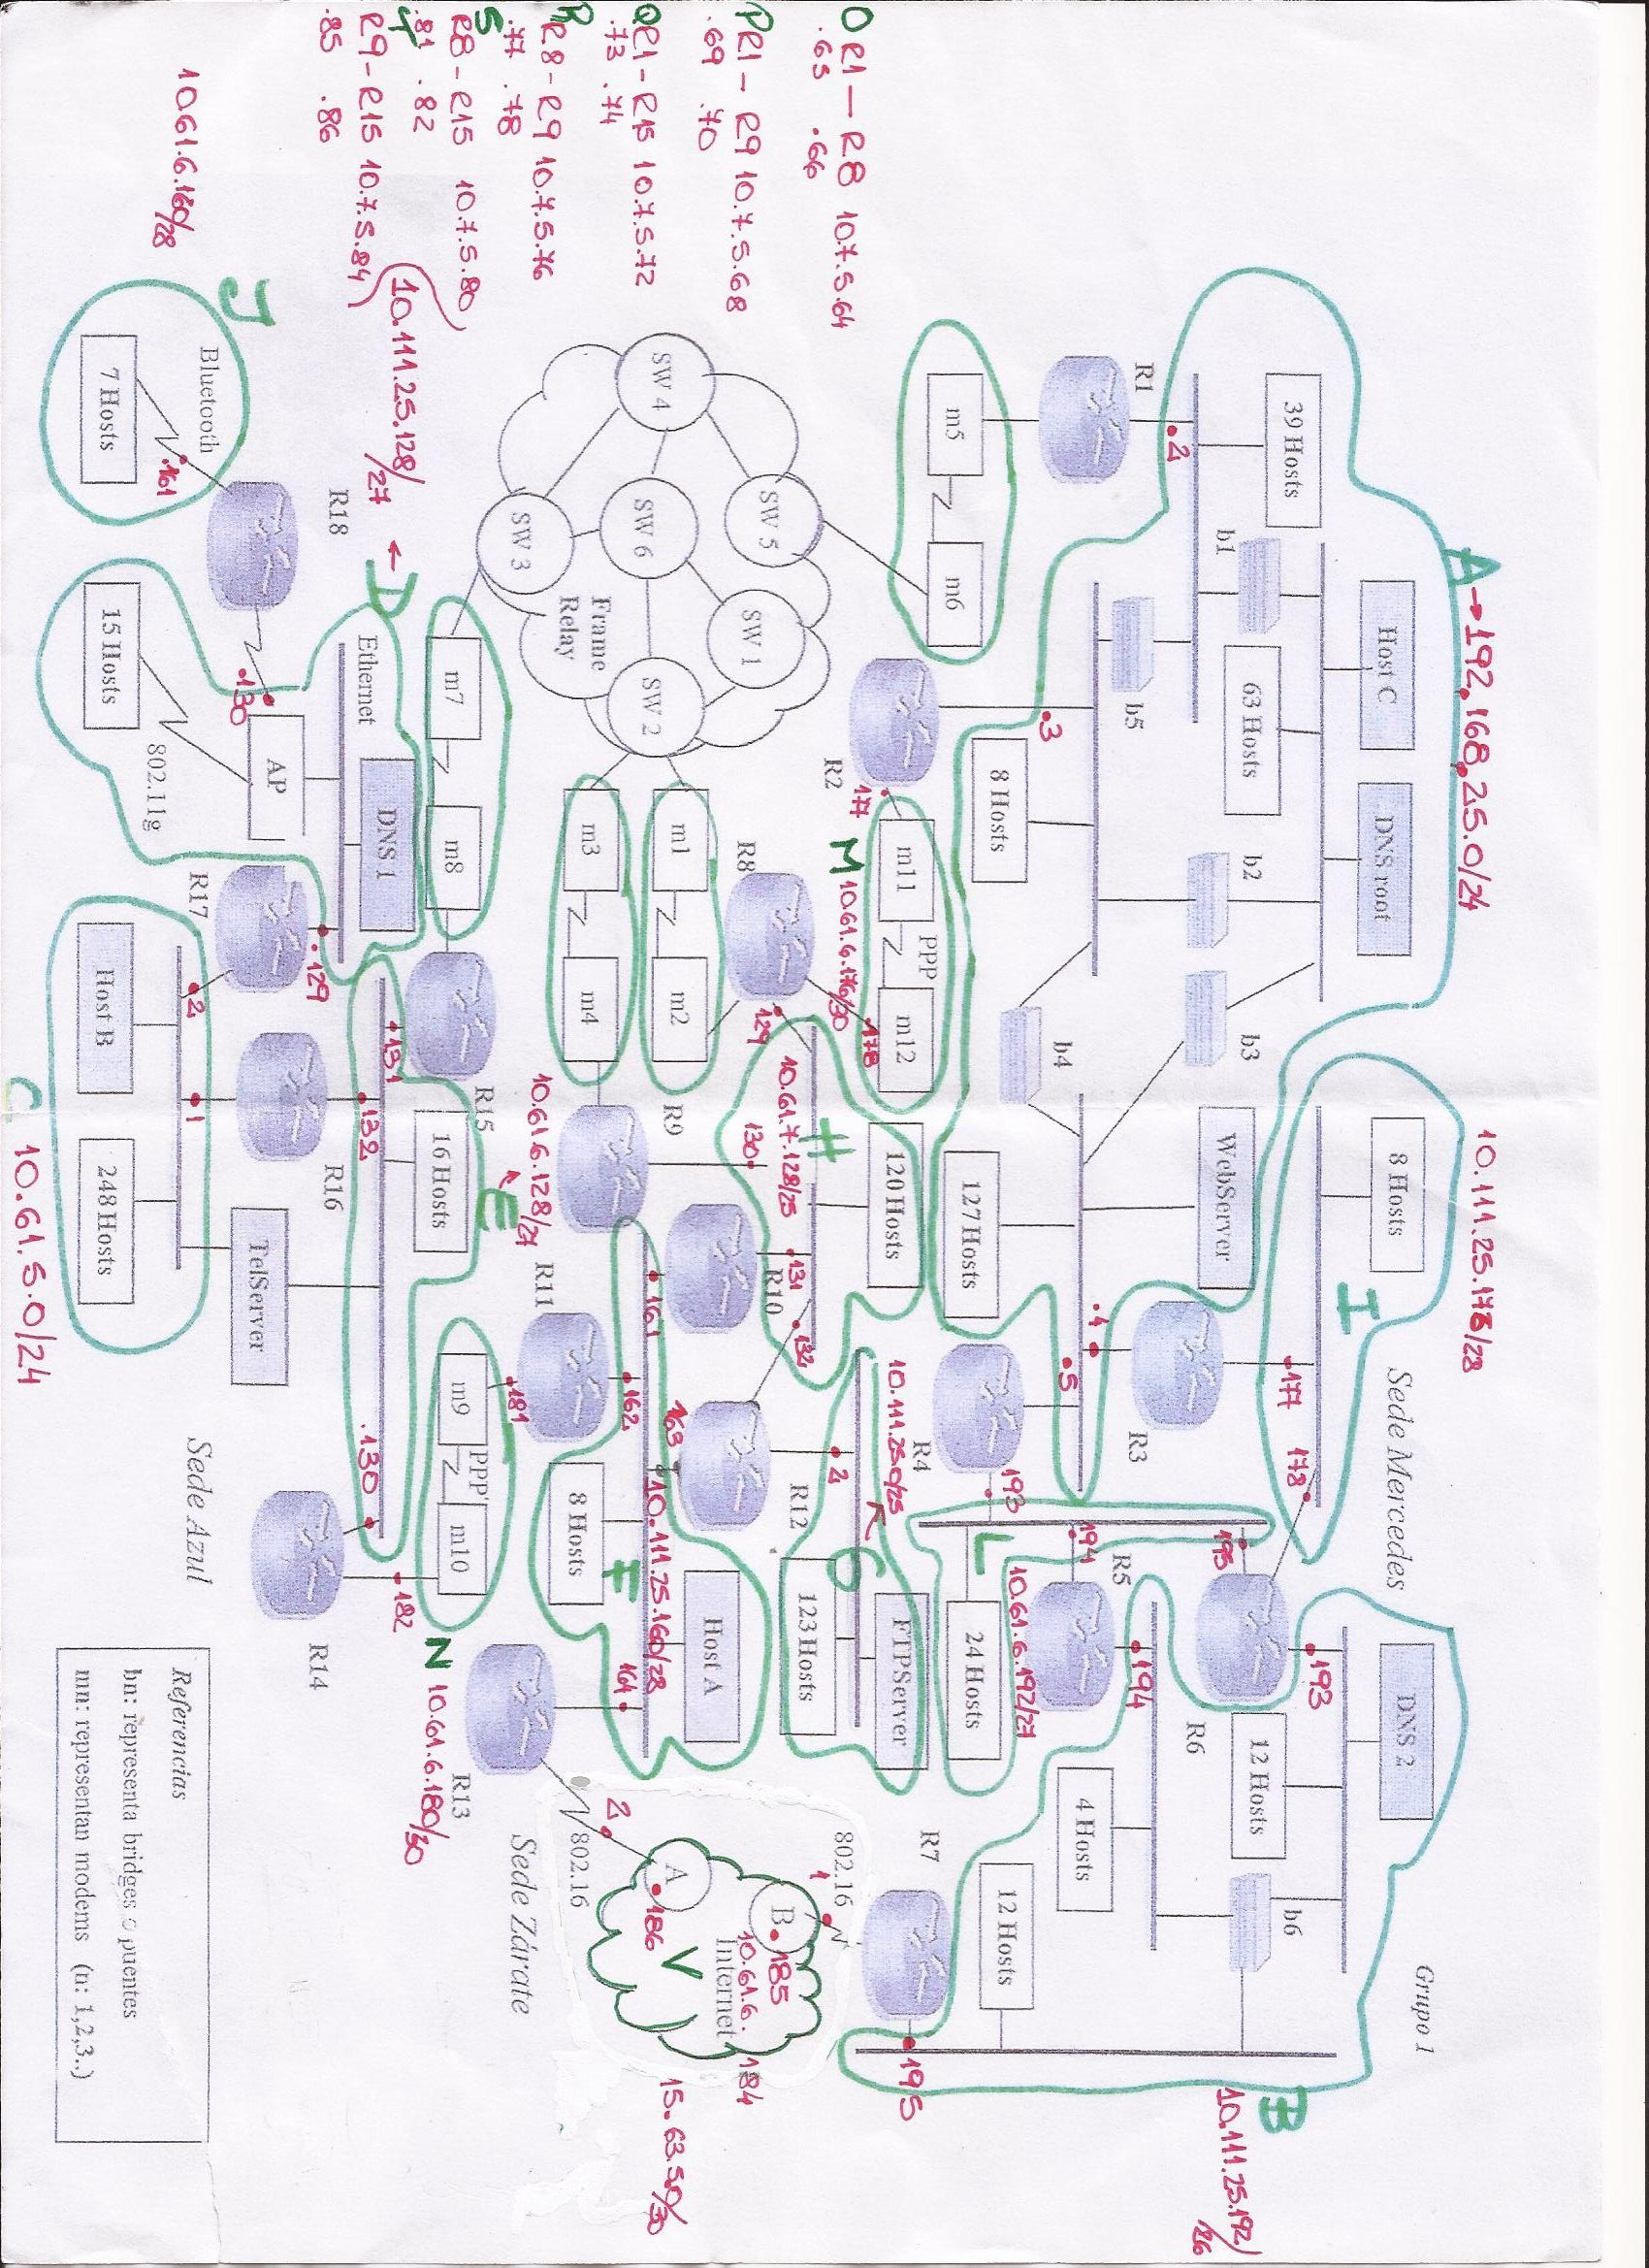
\includegraphics[width=13cm]{Imagenes/red.jpg}
      \end{center}
      \captionof{figure}{Diagrama de asignación de redes}
      \label{fig001}
\end{figure}

\begin{figure}[H]
      \centering
      \begin{center}
      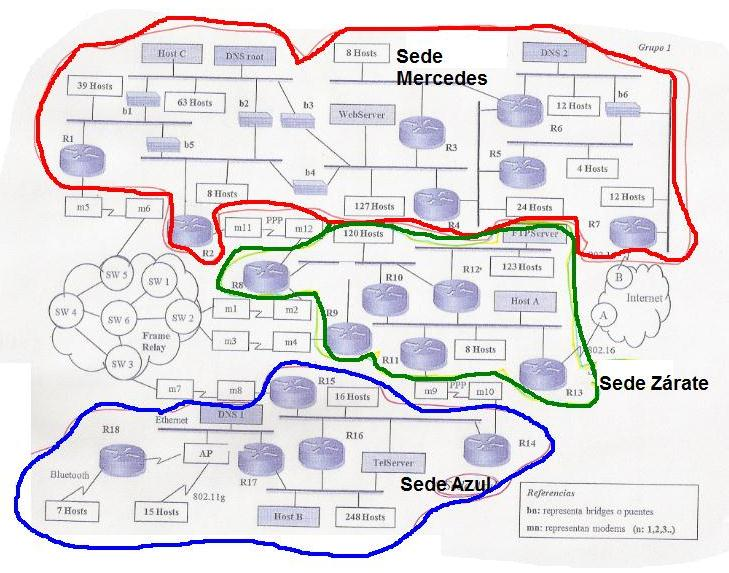
\includegraphics[width=1.2\textwidth]{Imagenes/sedes.jpg}
      \end{center}
      \captionof{figure}{Diagrama de delimitación de sedes}
      \label{fig002}
\end{figure}


La topología se divide en tres sedes: \textit{Azul, Mercedes y Zárate}. Es importante delimitar que redes pertenecen a cada sede
dado que de esto depende la resolución de nombres de dominios (DNS) y la aplicación de los protocolos de ruteo. En la figura \ref{fig002} se muestra 
la división de la red en las tres respectivas sedes. \\
\indent Con el espacio de direccionamiento asignado a cada red, se procedió a asignar las direcciones correspondientes a cada host perteneciente a las mismas. 
Las direcciones asignadas corresponden a las interfaces de los routers pertenecientes a la red y a los hosts especiales que se asignaron a las mismas
en la topología (Servers, DNSs o Hosts particulares). \\ 

\subsection{Amapola}

\textbf{Dirección de red:} 192.168.25.0/24

\begin{table}[!htbp]
\centering
  \begin{tabular}{|c|c|c|}
    \hline
	Router & Dirección & Dirección Virtual\\ \hline
	R1 & 192.168.25.2 &  - \\ \hline
	R2 & 192.168.25.3 &  - \\ \hline
	R3 & 192.168.25.4 & 192.168.25.6 \\ \hline
	R3 & 192.168.25.5 & 192.168.25.6 \\
    \hline
  \end{tabular}
  \captionof{table}{Tabla de asignación de routers en Amapola}
\end{table}

\begin{table}[!htbp]
\centering
  \begin{tabular}{|c|c|}
    \hline
	DNS Root & 192.168.25.7 \\ \hline
	Host C & 192.168.25.6 \\ \hline
	Web Server & 192.168.25.1 \\
    \hline
  \end{tabular}
  \captionof{table}{Tabla de asignaciones especiales de Amapola}
\end{table}

\subsection{Begonia}

\textbf{Dirección de red:} 10.111.25.192/26

\begin{table}[!htbp]
\centering
  \begin{tabular}{|c|c|c|}
    \hline
	Router & Dirección & Dirección Virtual\\ \hline
	R6 & 10.111.25.193 & 10.111.25.196 \\ \hline
	R7 & 10.111.25.194 & 10.111.25.196  \\ \hline
	R8 & 10.111.25.195 & - \\
    \hline
  \end{tabular}
  \captionof{table}{Tabla de asignación de routers en Begonia}
\end{table}

\begin{table}[!htbp]
\centering
  \begin{tabular}{|c|c|}
    \hline
	DNS2& 10.111.25.196 \\
    \hline
  \end{tabular}
  \captionof{table}{Tabla de asignaciones especiales de Begonia}
\end{table}

\subsection{Clavel}
\textbf{Dirección de red:} 10.61.5.0/24
\begin{table}[!htbp]
\centering
  \begin{tabular}{|c|c|}
    \hline
	Router & Dirección\\ \hline
	R16 & 10.61.5.1 \\ \hline
	R17 & 10.61.5.2 \\
    \hline
  \end{tabular}
  \captionof{table}{Tabla de asignación de routers en Clavel}
\end{table}

\begin{table}[!htbp]
\centering
  \begin{tabular}{|c|c|}
    \hline
	TelServer& 10.61.5.130 \\
    \hline
  \end{tabular}
  \captionof{table}{Tabla de asignaciones especiales de Clavel}
\end{table}

\subsection{Dalia}
\textbf{Dirección de red:} 10.111.25.128/27
\begin{table}[!htbp]
\centering
  \begin{tabular}{|c|c|}
    \hline
	Router & Dirección\\ \hline
	R17 & 10.111.25.129\\ \hline
	R18 & 10.111.25.130\\
    \hline
  \end{tabular}
  \captionof{table}{Tabla de asignación de routers en Dalia}
\end{table}

\begin{table}[!htbp]
\centering
  \begin{tabular}{|c|c|}
    \hline
	DNS1& 10.111.25.131 \\
    \hline
  \end{tabular}
  \captionof{table}{Tabla de asignaciones especiales de Dalia}
\end{table}

\subsection{Espuela}
\textbf{Dirección de red:} 10.61.6.128/27
\begin{table}[!htbp]
\centering
  \begin{tabular}{|c|c|}
    \hline
	Router & Dirección\\ \hline
	R14 & 10.61.6.130\\ \hline
	R15 & 10.61.6.131\\ \hline
	R16 & 10.61.6.132\\
    \hline
  \end{tabular}
  \captionof{table}{Tabla de asignación de routers en Espuela}
\end{table}

\begin{table}[!htbp]
\centering
  \begin{tabular}{|c|c|}
    \hline
	TelnetServer& 10.61.6.129 \\
    \hline
  \end{tabular}
  \captionof{table}{Tabla de asignaciones especiales de Espuela}
\end{table}

\subsection{Fresia}
\textbf{Dirección de red:} 10.111.25.160/28
\begin{table}[!htbp]
\centering
  \begin{tabular}{|c|c|}
    \hline
	Router & Dirección\\ \hline
	R10 & 10.111.25.161\\ \hline
	R11 & 10.111.25.162\\ \hline
	R12 & 10.111.25.163\\ \hline
	R13 & 10.111.25.164\\
    \hline
  \end{tabular}
  \captionof{table}{Tabla de asignación de routers en Fresia}
\end{table}

\begin{table}[!htbp]
\centering
  \begin{tabular}{|c|c|}
    \hline
	Host A&10.111.25.165\\
    \hline
  \end{tabular}
  \captionof{table}{Tabla de asignaciones especiales de Fresia}
\end{table}


\subsection{Geranio}
\textbf{Dirección de red:} 10.111.25.0/25
\begin{table}[!htbp]
\centering
  \begin{tabular}{|c|c|}
    \hline
	Router & Dirección\\ \hline
	R12 & 10.111.25.2\\
    \hline
  \end{tabular}
  \captionof{table}{Tabla de asignación de routers en Geranio}
\end{table}

\begin{table}[!htbp]
\centering
  \begin{tabular}{|c|c|}
    \hline
	FTP Server& 10.111.25.1\\
    \hline
  \end{tabular}
  \captionof{table}{Tabla de asignaciones especiales de Geranio}
\end{table}

\subsection{Hortensia}
\textbf{Dirección de red:} 10.61.7.128/25
\begin{table}[!htbp]
\centering
  \begin{tabular}{|c|c|}
    \hline
	Router & Dirección\\ \hline
	R8 & 10.61.7.129\\ \hline
	R9 & 10.61.7.130\\ \hline
	R10 & 10.61.7.131\\ \hline
	R12 & 10.61.7.132\\
    \hline
  \end{tabular}
  \captionof{table}{Tabla de asignación de routers en Hortensia}
\end{table}

\begin{table}[!htbp]
\centering
  \begin{tabular}{|c|c|}
    \hline
	TelnetServer& 10.61.6.129 \\
    \hline
  \end{tabular}
  \captionof{table}{Tabla de asignaciones especiales de Hortensia}
\end{table}

\subsection{Iris}
\textbf{Dirección de red:} 10.111.25.176/28
\begin{table}[!htbp]
\centering
  \begin{tabular}{|c|c|}
    \hline
	Router & Dirección\\ \hline
	R3 & 10.111.25.177\\ \hline
	R6 & 10.111.25.178\\
    \hline
  \end{tabular}
  \captionof{table}{Tabla de asignación de routers en Iris}
\end{table}

\subsection{Jazmín}
\textbf{Dirección de red:} 10.61.6.160/28
\begin{table}[!htbp]
\centering
  \begin{tabular}{|c|c|}
    \hline
	Router & Dirección\\ \hline
	R18 & 10.61.6.161\\
    \hline
  \end{tabular}
  \captionof{table}{Tabla de asignación de routers en Jazmín}
\end{table}

\subsection{Kentia}
\textbf{Dirección de red:} 157.63.5.0/30	
\begin{table}[!htbp]
\centering
  \begin{tabular}{|c|c|}
    \hline
	Router & Dirección\\ \hline
	R7 & 157.63.5.1\\ 
    \hline
  \end{tabular}
  \captionof{table}{Tabla de asignación de routers en Kentia}
\end{table}

\begin{table}[!htbp]
\centering
  \begin{tabular}{|c|c|}
    \hline
	Internet& 157.63.5.2 \\
    \hline
  \end{tabular}
  \captionof{table}{Tabla de asignaciones especiales de Kentia}
\end{table}

\subsection{Lirio}

\textbf{Dirección de red:} 10.61.6.192/27

\begin{table}[!htbp]
\centering
  \begin{tabular}{|c|c|c|}
    \hline
	Router & Dirección & Dirección Virtual\\ \hline
	R4 & 10.61.6.193 &  - \\ \hline
	R5 & 10.61.6.194 & 10.61.6.196  \\ \hline
	R6 & 10.61.6.195 & 10.61.6.196 \\
    \hline
  \end{tabular}
  \captionof{table}{Tabla de asignación de routers en Lirio}
\end{table}

\subsection{Margarita}
\textbf{Dirección de red:} 10.61.6.176/30
\begin{table}[!htbp]
\centering
  \begin{tabular}{|c|c|}
    \hline
	Router & Dirección\\ \hline
	R2 & 10.61.6.177\\ \hline
	R8 & 10.61.6.178\\
    \hline
  \end{tabular}
  \captionof{table}{Tabla de asignación de routers en Margarita}
\end{table}

\subsection{Narciso}
\textbf{Dirección de red:} 10.61.6.180/30
\begin{table}[!htbp]
\centering
  \begin{tabular}{|c|c|}
    \hline
	Router & Dirección\\ \hline
	R11 & 10.61.6.181\\ \hline
	R14 & 10.61.6.182\\
    \hline
  \end{tabular}
  \captionof{table}{Tabla de asignación de routers en Narciso}
\end{table}

\subsection{Orquídea}
\textbf{Dirección de red:} 10.7.5.64/30
\begin{table}[!htbp]
\centering
  \begin{tabular}{|c|c|}
    \hline
	Router & Dirección\\ \hline
	R1 & 10.7.5.65\\ \hline
	R8 &10.7.5.66\\
    \hline
  \end{tabular}
  \captionof{table}{Tabla de asignación de routers en Orquídea}
\end{table}

\subsection{Petunia}
\textbf{Dirección de red:} 10.7.5.68/30
\begin{table}[!htbp]
\centering
  \begin{tabular}{|c|c|}
    \hline
	Router & Dirección\\ \hline
	R1 &10.7.5.69\\ \hline
	R9 &10.7.5.70\\
    \hline
  \end{tabular}
  \captionof{table}{Tabla de asignación de routers en Petunia}
\end{table}

\subsection{Quimonant}
\textbf{Dirección de red:} 10.7.5.72/30
\begin{table}[!htbp]
\centering
  \begin{tabular}{|c|c|}
    \hline
	Router & Dirección\\ \hline
	R1 &10.7.5.73\\ \hline
	R15 &10.7.5.74\\
    \hline
  \end{tabular}
  \captionof{table}{Tabla de asignación de routers en Quimonant}
\end{table}

\subsection{Rosa}
\textbf{Dirección de red:} 10.7.5.76/30
\begin{table}[!htbp]
\centering
  \begin{tabular}{|c|c|}
    \hline
	Router & Dirección\\ \hline
	R8 &10.7.5.77\\ \hline
	R9 &10.7.5.78\\
    \hline
  \end{tabular}
  \captionof{table}{Tabla de asignación de routers en Rosa}
\end{table}


\subsection{Siempreviva}
\textbf{Dirección de red:} 10.7.5.80/30
\begin{table}[!htbp]
\centering
  \begin{tabular}{|c|c|}
    \hline
	Router & Dirección\\ \hline
	R8 &10.7.5.81\\ \hline
	R15 &10.7.5.82\\
    \hline
  \end{tabular}
  \captionof{table}{Tabla de asignación de routers en Siempreviva}
\end{table}

\subsection{Tulipán}
\textbf{Dirección de red:} 10.7.5.84/30
\begin{table}[!htbp]
\centering
  \begin{tabular}{|c|c|}
    \hline
	Router & Dirección\\ \hline
	R9 &10.7.5.85\\ \hline
	R15 &10.7.5.86\\
    \hline
  \end{tabular}
  \captionof{table}{Tabla de asignación de routers en Tulipán}
\end{table}

\subsection{Ulmaria}
\textbf{Dirección de red:} 157.63.5.4/30	
\begin{table}[!htbp]
\centering
  \begin{tabular}{|c|c|}
    \hline
	Router & Dirección\\ \hline
	R13 & 157.63.5.6\\ 
	\hline
  \end{tabular}
  \captionof{table}{Tabla de asignación de routers en Ulmaria}
\end{table}

\begin{table}[!htbp]
\centering
  \begin{tabular}{|c|c|}
    \hline
	Internet& 157.63.5.5 \\
    \hline
  \end{tabular}
  \captionof{table}{Tabla de asignaciones especiales de Ulmaria}
\end{table}

\subsection{Violeta}
\textbf{Dirección de red:} 10.61.6.184/30
\begin{table}[!htbp]
\centering
  \begin{tabular}{|c|c|}
    \hline
	Router & Dirección\\ \hline
	R7 &10.61.6.185\\ \hline
	R13 &10.61.6.186\\
    \hline
  \end{tabular}
  \captionof{table}{Tabla de asignación de routers en Violeta}
\end{table}


\newpage
\section{Ruteo}
En esta sección se muestran los diferentes tipos de ruteos aplicados a cada parte de la red. En el caso de 
ruteo estático, se muestran las tablas de ruteo de los routers en cuestión. En el caso de ruteo dinámico, 
se da una breve explicación del funcionamiento del protocolo de ruteo utilizado y los comandos necesarios
para configurar al mismo.

\subsection{Ruteo Estático - Rutas Principales}
Para establecer las tablas de ruteo se optó por diseñar un cámino mínimo aproximado, eligiendo 
de forma arbitraria la ruta en caso de empate. A continuación se muestran los resultados obtenidos 
para cada router, omitiendo a aquellos routers en los cuales se aplica únicamente ruteo dinámico (son los 
routers correspondientes a la sede Mercedes, R3, R4, R5 y R6). Los routers R1, R2
y R7 poseen interfaces que se comunican tanto con la sede Mercedes como con la sede Zárate, de forma que la
tabla de ruteo de los mismos poseerán entradas estáticas como dinámicas. Sin embargo, en esta subsección sólo 
se muestran las entradas estáticas.

\subsubsection{R1}
\begin{table}[!htbp]
\centering
  \begin{tabular}{|c|c|c|c|}
    \hline
	Red & Dirección de red & Mascara & Next Hop\\ \hline
	C & 10.61.5.0 & 255.255.255.0 & 10.7.5.74   \\ \hline
	D & 10.111.25.128 & 255.255.255.224 & 10.7.5.74 \\ \hline
	E & 10.61.6.128 & 255.255.255.224 & 10.7.5.74 \\ \hline
	F & 10.111.25.160 & 255.255.255.240 & 10.7.5.66 \\ \hline
	G & 10.111.25.0 & 255.255.255.128 & 10.7.5.66 \\ \hline
	H & 10.61.7.128 & 255.255.255.128 & 10.7.5.66 \\ \hline
	J & 10.61.6.160 & 255.255.255.240 & 10.7.5.74 \\ \hline
	M & 10.61.6.176 & 255.255.255.252 & 10.7.5.66 \\ \hline
	N & 10.61.6.180 & 255.255.255.252 & 10.7.5.74 \\ \hline
	R & 10.7.5.76 & 255.255.255.252 & 10.7.5.66 \\ \hline
	S & 10.7.5.80 & 255.255.255.252 & 10.7.5.74 \\ \hline
	T & 10.7.5.84 & 255.255.255.252 & 10.7.5.74 \\ \hline
	V & 10.61.6.184 & 255.255.255.252 & 10.7.5.66 \\
    \hline
  \end{tabular}
  \captionof{table}{Tabla de ruteo R1}
\end{table}

\newpage
\subsubsection{R2}
\begin{table}[!htbp]
\centering
  \begin{tabular}{|c|c|c|c|}
    \hline
	Red & Dirección de red & Mascara & Next Hop\\ \hline
	C & 10.61.5.0 & 255.255.255.0 & 10.61.6.178 \\ \hline
	D & 10.111.25.128 & 255.255.255.224 & 10.61.6.178 \\ \hline
	E & 10.61.6.128 & 255.255.255.224 & 10.61.6.178 \\ \hline
	F & 10.111.25.160 & 255.255.255.240 & 10.61.6.178 \\ \hline
	G & 10.111.25.0 & 255.255.255.128 & 10.61.6.178 \\ \hline
	H & 10.61.7.128 & 255.255.255.128 & 10.61.6.178 \\ \hline
	J & 10.61.6.160 & 255.255.255.240 & 10.61.6.178 \\ \hline
	M & 10.61.6.176 & 255.255.255.252 & 10.61.6.178 \\ \hline
	N & 10.61.6.180 & 255.255.255.252 & 10.61.6.178 \\ \hline
	O & 10.7.5.64 & 255.255.255.252 & 10.61.6.178 \\ \hline
	P & 10.7.5.68 & 255.255.255.252 & 10.61.6.178 \\ \hline
	Q & 10.7.5.72 & 255.255.255.252 & 10.61.6.178 \\ \hline
	R & 10.7.5.76 & 255.255.255.252 & 10.61.6.178 \\ \hline
	S & 10.7.5.80 & 255.255.255.252 & 10.61.6.178 \\ \hline
	T & 10.7.5.84 & 255.255.255.252 & 10.61.6.178 \\ \hline
	V & 10.61.6.184 & 255.255.255.252 & 10.61.6.178 \\
    \hline
  \end{tabular}
  \captionof{table}{Tabla de ruteo R2}
\end{table}

\newpage
\subsubsection{R7}
\begin{table}[!htbp]
\centering
  \begin{tabular}{|c|c|c|c|}
    \hline
	Red & Dirección de red & Mascara & Next Hop\\ \hline
	C & 10.61.5.0 & 255.255.255.0 & Tunel 10: 10.61.6.186 \\ \hline
	D & 10.111.25.128 & 255.255.255.224 & Tunel 10: 10.61.6.186 \\ \hline
	E & 10.61.6.128 & 255.255.255.224 & Tunel 10: 10.61.6.186 \\ \hline
	F & 10.111.25.160 & 255.255.255.240 & Tunel 10: 10.61.6.186 \\ \hline
	G & 10.111.25.0 & 255.255.255.128 & Tunel 10: 10.61.6.186 \\ \hline
	H & 10.61.7.128 & 255.255.255.128 & Tunel 10: 10.61.6.186 \\ \hline
	J & 10.61.6.160 & 255.255.255.240 & Tunel 10: 10.61.6.186 \\ \hline
	M & 10.61.6.176 & 255.255.255.252 & Tunel 10: 10.61.6.186 \\ \hline
	N & 10.61.6.180 & 255.255.255.252 & Tunel 10: 10.61.6.186 \\ \hline
	O & 10.7.5.64 & 255.255.255.252 & Tunel 10: 10.61.6.186 \\ \hline
	P & 10.7.5.68 & 255.255.255.252 & Tunel 10: 10.61.6.186 \\ \hline
	Q & 10.7.5.72 & 255.255.255.252 & Tunel 10: 10.61.6.186 \\ \hline
	R & 10.7.5.76 & 255.255.255.252 & Tunel 10: 10.61.6.186 \\ \hline
	S & 10.7.5.80 & 255.255.255.252 & Tunel 10: 10.61.6.186 \\ \hline
	T & 10.7.5.84 & 255.255.255.252 & Tunel 10: 10.61.6.186 \\ \hline
	V & 10.61.6.184 & 255.255.255.252 & Tunel 10: 10.61.6.186 \\
    \hline
  \end{tabular}
  \captionof{table}{Tabla de ruteo R7}
\end{table}

\newpage
\subsubsection{R8}
\begin{table}[!htbp]
\centering
  \begin{tabular}{|c|c|c|c|}
    \hline
	Red & Dirección de red & Mascara & Next Hop\\ \hline
	A & 192.168.25.0 & 255.255.255.0 & 10.61.6.177 \\ \hline
	B & 10.111.25.192 & 255.255.255.192 & 10.61.6.177 \\ \hline
	C & 10.61.5.0 & 255.255.255.0 & 10.7.5.82 \\ \hline
	D & 10.111.25.128 & 255.255.255.224 & 10.7.5.82 \\ \hline
	E & 10.61.6.128 & 255.255.255.224 & 10.7.5.82 \\ \hline
	F & 10.111.25.160 & 255.255.255.240 & 10.61.7.131 \\ \hline
	G & 10.111.25.0 & 255.255.255.128 & 10.61.7.132 \\ \hline
	I & 10.111.25.176 & 255.255.255.240 & 10.61.6.177 \\ \hline
	J & 10.61.6.160 & 255.255.255.240 & 10.7.5.82 \\ \hline
	L & 10.61.6.192 & 255.255.255.224 & 10.61.6.177 \\ \hline
	N & 10.61.6.180 & 255.255.255.252 & 10.7.5.82 \\ \hline
	P & 10.7.5.68 & 255.255.255.252 & 10.7.5.65 \\ \hline
	Q & 10.7.5.72 & 255.255.255.252 & 10.7.5.65 \\ \hline
	T & 10.7.5.84 & 255.255.255.252 & 10.7.5.82 \\ \hline
	V & 10.61.6.184 & 255.255.255.252 & 10.61.7.132 \\
    \hline
  \end{tabular}
  \captionof{table}{Tabla de ruteo R8}
\end{table}

\newpage
\subsubsection{R9}
\begin{table}[!htbp]
\centering
  \begin{tabular}{|c|c|c|c|}
    \hline
	Red & Dirección de red & Mascara & Next Hop\\ \hline
	A & 192.168.25.0 & 255.255.255.0 & 10.7.5.65 \\ \hline
	B & 10.111.25.192 & 255.255.255.192 & 10.7.5.65 \\ \hline
	C & 10.61.5.0 & 255.255.255.0 & 10.7.5.86 \\ \hline
	D & 10.111.25.128 & 255.255.255.224 & 10.7.5.86 \\ \hline
	E & 10.61.6.128 & 255.255.255.224 & 10.7.5.86 \\ \hline
	F & 10.111.25.160 & 255.255.255.240 & 10.61.7.131 \\ \hline
	G & 10.111.25.0 & 255.255.255.128 & 10.61.7.132 \\ \hline
	I & 10.111.25.176 & 255.255.255.240 & 10.7.5.65 \\ \hline
	J & 10.61.6.160 & 255.255.255.240 & 10.7.5.86 \\ \hline
	L & 10.61.6.192 & 255.255.255.224 & 10.7.5.65 \\ \hline
	M & 10.61.6.176 & 255.255.255.252 & 10.7.5.77 \\ \hline
	N & 10.61.6.180 & 255.255.255.252 & 10.7.5.86 \\ \hline
	O & 10.7.5.64 & 255.255.255.252 & 10.7.5.77 \\ \hline
	P & 10.7.5.68 & 255.255.255.252 & 10.61.7.130 \\ \hline
	Q & 10.7.5.72 & 255.255.255.252 & 10.7.5.86 \\ \hline
	S & 10.7.5.80 & 255.255.255.252 & 10.7.5.77 \\ \hline
	V & 10.61.6.184 & 255.255.255.252 & 10.61.7.132 \\
    \hline
  \end{tabular}
  \captionof{table}{Tabla de ruteo R9}
\end{table}

\newpage
\subsubsection{R10}
\begin{table}[!htbp]
\centering
  \begin{tabular}{|c|c|c|c|}
    \hline
	Red & Dirección de red & Mascara & Next Hop\\ \hline
	A & 192.168.25.0 & 255.255.255.0 & 10.61.7.129 \\ \hline
	B & 10.111.25.192 & 255.255.255.192 & 10.111.25.164 \\ \hline
	C & 10.61.5.0 & 255.255.255.0 & 10.61.7.130 \\ \hline
	D & 10.111.25.128 & 255.255.255.224 & 10.61.7.130 \\ \hline
	E & 10.61.6.128 & 255.255.255.224 & 10.61.7.130 \\ \hline
	G & 10.111.25.0 & 255.255.255.128 & 10.61.7.132 \\ \hline
	I & 10.111.25.176 & 255.255.255.240 & 10.61.7.129 \\ \hline
	J & 10.61.6.160 & 255.255.255.240 & 10.61.7.130 \\ \hline
	L & 10.61.6.192 & 255.255.255.224 & 10.61.7.129 \\ \hline
	M & 10.61.6.176 & 255.255.255.252 & 10.61.7.129 \\ \hline
	N & 10.61.6.180 & 255.255.255.252 & 10.111.25.162 \\ \hline
	O & 10.7.5.64 & 255.255.255.252 & 10.61.7.129 \\ \hline
	P & 10.7.5.68 & 255.255.255.252 & 10.61.7.130 \\ \hline
	Q & 10.7.5.72 & 255.255.255.252 & 10.61.7.130 \\ \hline
	R & 10.7.5.76 & 255.255.255.252 & 10.61.7.130 \\ \hline
	S & 10.7.5.80 & 255.255.255.252 & 10.61.7.129 \\ \hline
	T & 10.7.5.84 & 255.255.255.252 & 10.61.7.130 \\ \hline
	V & 10.61.6.184 & 255.255.255.252 & 10.111.25.164 \\
    \hline
  \end{tabular}
  \captionof{table}{Tabla de ruteo R10}
\end{table}

\newpage
\subsubsection{R11}
\begin{table}[!htbp]
\centering
  \begin{tabular}{|c|c|c|c|}
    \hline
	Red & Dirección de red & Mascara & Next Hop\\ \hline
	A & 192.168.25.0 & 255.255.255.0 & 10.111.25.161 \\ \hline
	B & 10.111.25.192 & 255.255.255.192 & 10.111.25.164 \\ \hline
	C & 10.61.5.0 & 255.255.255.0 & 10.61.6.182 \\ \hline
	D & 10.111.25.128 & 255.255.255.224 & 10.61.6.182 \\ \hline
	E & 10.61.6.128 & 255.255.255.224 & 10.61.6.182 \\ \hline
	G & 10.111.25.0 & 255.255.255.128 & 10.111.25.163 \\ \hline
	H & 10.61.7.128 & 255.255.255.128 & 10.111.25.161 \\ \hline
	I & 10.111.25.176 & 255.255.255.240 & 10.111.25.161 \\ \hline
	J & 10.61.6.160 & 255.255.255.240 & 10.61.6.182 \\ \hline
	L & 10.61.6.192 & 255.255.255.224 & 10.111.25.161 \\ \hline
	M & 10.61.6.176 & 255.255.255.252 & 10.111.25.163 \\ \hline
	O & 10.7.5.64 & 255.255.255.252 & 10.111.25.163 \\ \hline
	P & 10.7.5.68 & 255.255.255.252 & 10.111.25.163 \\ \hline
	Q & 10.7.5.72 & 255.255.255.252 & 10.61.6.182 \\ \hline
	R & 10.7.5.76 & 255.255.255.252 & 10.111.25.163 \\ \hline
	S & 10.7.5.80 & 255.255.255.252 & 10.61.6.182 \\ \hline
	T & 10.7.5.84 & 255.255.255.252 & 10.61.6.182 \\ \hline
	V & 10.61.6.184 & 255.255.255.252 & 10.111.25.164 \\
    \hline
  \end{tabular}
  \captionof{table}{Tabla de ruteo R11}
\end{table}

\newpage
\subsubsection{R12}
\begin{table}[!htbp]
\centering
  \begin{tabular}{|c|c|c|c|}
    \hline
	Red & Dirección de red & Mascara & Next Hop\\ \hline
	A & 192.168.25.0 & 255.255.255.0 & 10.61.7.129 \\ \hline
	B & 10.111.25.192 & 255.255.255.192 & 10.111.25.164 \\ \hline
	C & 10.61.5.0 & 255.255.255.0 & 10.111.25.162 \\ \hline
	D & 10.111.25.128 & 255.255.255.224 & 10.111.25.162 \\ \hline
	E & 10.61.6.128 & 255.255.255.224 & 10.111.25.162 \\ \hline
	I & 10.111.25.176 & 255.255.255.240 & 10.61.7.129 \\ \hline
	J & 10.61.6.160 & 255.255.255.240 & 10.111.25.162 \\ \hline
	L & 10.61.6.192 & 255.255.255.224 & 10.111.25.164 \\ \hline
	M & 10.61.6.176 & 255.255.255.252 & 10.61.7.129 \\ \hline
	N & 10.61.6.180 & 255.255.255.252 & 10.111.25.162 \\ \hline
	O & 10.7.5.64 & 255.255.255.252 & 10.61.7.129 \\ \hline
	P & 10.7.5.68 & 255.255.255.252 & 10.61.7.130 \\ \hline
	Q & 10.7.5.72 & 255.255.255.252 & 10.61.7.129 \\ \hline
	R & 10.7.5.76 & 255.255.255.252 & 10.61.7.129 \\ \hline
	S & 10.7.5.80 & 255.255.255.252 & 10.61.7.129 \\ \hline
	T & 10.7.5.84 & 255.255.255.252 & 10.61.7.130 \\ \hline
	V & 10.61.6.184 & 255.255.255.252 & 10.111.25.164 \\
    \hline
  \end{tabular}
  \captionof{table}{Tabla de ruteo R12}
\end{table}

\newpage
\subsubsection{R13}
\begin{table}[!htbp]
\centering
  \begin{tabular}{|c|c|c|c|}
    \hline
	Red & Dirección de red & Mascara & Next Hop\\ \hline
	A & 192.168.25.0 & 255.255.255.0 & 10.111.25.161 \\ \hline
	B & 10.111.25.192 & 255.255.255.192 & Tunnel 20:10.61.6.185 \\ \hline
	C & 10.61.5.0 & 255.255.255.0 & 10.111.25.162 \\ \hline
	D & 10.111.25.128 & 255.255.255.224 & 10.111.25.162 \\ \hline
	E & 10.61.6.128 & 255.255.255.224 & 10.111.25.162 \\ \hline
	F & 10.111.25.160 & 255.255.255.240 & 10.111.25.163 \\ \hline
	G & 10.111.25.0 & 255.255.255.128 & 10.111.25.163 \\ \hline
	H & 10.61.7.128 & 255.255.255.128 & 10.111.25.161 \\ \hline
	I & 10.111.25.176 & 255.255.255.240 & Tunel 20: 10.61.6.185 \\ \hline
	J & 10.61.6.160 & 255.255.255.240 & 10.111.25.162 \\ \hline
	L & 10.61.6.192 & 255.255.255.224 & Tunel 20: 10.61.6.185 \\ \hline
	M & 10.61.6.176 & 255.255.255.252 & 10.111.25.161 \\ \hline
	N & 10.61.6.180 & 255.255.255.252 & 10.111.25.162 \\ \hline
	O & 10.7.5.64 & 255.255.255.252 & 10.111.25.163 \\ \hline
	P & 10.7.5.68 & 255.255.255.252 & 10.111.25.163 \\ \hline
	Q & 10.7.5.72 & 255.255.255.252 & 10.111.25.162 \\ \hline
	R & 10.7.5.76 & 255.255.255.252 & 10.111.25.161 \\ \hline
	S & 10.7.5.80 & 255.255.255.252 & 10.111.25.161 \\ \hline
	T & 10.7.5.84 & 255.255.255.252 & 10.111.25.161 \\ \hline
    \hline
  \end{tabular}
  \captionof{table}{Tabla de ruteo R13}
\end{table}

\newpage
\subsubsection{R14}
\begin{table}[!htbp]
\centering
  \begin{tabular}{|c|c|c|c|}
    \hline
	Red & Dirección de red & Mascara & Next Hop\\ \hline
	A & 192.168.25.0 & 255.255.255.0 & 10.61.6.131 \\ \hline
	B & 10.111.25.192 & 255.255.255.192 & 10.61.6.181 \\ \hline
	C & 10.61.5.0 & 255.255.255.0 & 10.61.6.132 \\ \hline
	D & 10.111.25.128 & 255.255.255.224 & 10.61.6.132 \\ \hline
	F & 10.111.25.160 & 255.255.255.240 & 10.61.6.181 \\ \hline
	G & 10.111.25.0 & 255.255.255.128 & 10.61.6.181 \\ \hline
	H & 10.61.7.128 & 255.255.255.128 & 10.61.6.181 \\ \hline
	I & 10.111.25.176 & 255.255.255.240 & 10.61.6.131 \\ \hline
	J & 10.61.6.160 & 255.255.255.240 & 10.61.6.132 \\ \hline
	L & 10.61.6.192 & 255.255.255.224 & 10.61.6.131 \\ \hline
	M & 10.61.6.176 & 255.255.255.252 & 10.61.6.131 \\ \hline
	O & 10.7.5.64 & 255.255.255.252 & 10.61.6.131 \\ \hline
	P & 10.7.5.68 & 255.255.255.252 & 10.61.6.131 \\ \hline
	Q & 10.7.5.72 & 255.255.255.252 & 10.61.6.131 \\ \hline
	R & 10.7.5.76 & 255.255.255.252 & 10.61.6.131 \\ \hline
	S & 10.7.5.80 & 255.255.255.252 & 10.61.6.131 \\ \hline
	T & 10.7.5.84 & 255.255.255.252 & 10.61.6.131 \\ \hline
	V & 10.61.6.184 & 255.255.255.252 & 10.61.6.181 \\
    \hline
  \end{tabular}
  \captionof{table}{Tabla de ruteo R14}
\end{table}

\newpage
\subsubsection{R15}
\begin{table}[!htbp]
\centering
  \begin{tabular}{|c|c|c|c|}
    \hline
	Red & Dirección de red & Mascara & Next Hop\\ \hline
	A & 192.168.25.0 & 255.255.255.0 & 10.7.5.73 \\ \hline
	B & 10.111.25.192 & 255.255.255.192 & 10.7.5.73 \\ \hline
	C & 10.61.5.0 & 255.255.255.0 & 10.61.6.132 \\ \hline
	D & 10.111.25.128 & 255.255.255.224 & 10.61.6.132 \\ \hline
	F & 10.111.25.160 & 255.255.255.240 & 10.7.5.85 \\ \hline
	G & 10.111.25.0 & 255.255.255.128 & 10.7.5.81 \\ \hline
	H & 10.61.7.128 & 255.255.255.128 & 10.7.5.81 \\ \hline
	I & 10.111.25.176 & 255.255.255.240 & 10.7.5.73 \\ \hline
	J & 10.61.6.160 & 255.255.255.240 & 10.61.6.132 \\ \hline
	L & 10.61.6.192 & 255.255.255.224 & 10.7.5.73 \\ \hline
	M & 10.61.6.176 & 255.255.255.252 & 10.7.5.81 \\ \hline
	N & 10.61.6.180 & 255.255.255.252 & 10.61.6.130 \\ \hline
	O & 10.7.5.64 & 255.255.255.252 & 10.7.5.73 \\ \hline
	P & 10.7.5.68 & 255.255.255.252 & 10.7.5.85 \\ \hline
	R & 10.7.5.76 & 255.255.255.252 & 10.7.5.81 \\ \hline
	V & 10.61.6.184 & 255.255.255.252 & 10.61.6.130 \\
    \hline
  \end{tabular}
  \captionof{table}{Tabla de ruteo R15}
\end{table}

\newpage
\subsubsection{R16}
\begin{table}[!htbp]
\centering
  \begin{tabular}{|c|c|c|c|}
    \hline
	Red & Dirección de red & Mascara & Next Hop\\ \hline
	A & 192.168.25.0 & 255.255.255.0 & 10.61.6.131 \\ \hline
	B & 10.111.25.192 & 255.255.255.192 & 10.61.6.130 \\ \hline
	D & 10.111.25.128 & 255.255.255.224 & 10.61.5.2 \\ \hline
	F & 10.111.25.160 & 255.255.255.240 & 10.61.6.130 \\ \hline
	G & 10.111.25.0 & 255.255.255.128 & 10.61.6.130 \\ \hline
	H & 10.61.7.128 & 255.255.255.128 & 10.61.6.131 \\ \hline	
	I & 10.111.25.176 & 255.255.255.240 & 10.61.6.131 \\ \hline
	J & 10.61.6.160 & 255.255.255.240 & 10.61.5.2 \\ \hline
	L & 10.61.6.192 & 255.255.255.224 & 10.61.6.131 \\ \hline
	M & 10.61.6.176 & 255.255.255.252 & 10.61.6.131 \\ \hline
	N & 10.61.6.180 & 255.255.255.252 & 10.61.6.130 \\ \hline
	O & 10.7.5.64 & 255.255.255.252 & 10.61.6.131 \\ \hline
	P & 10.7.5.68 & 255.255.255.252 & 10.61.6.131 \\ \hline
	Q & 10.7.5.72 & 255.255.255.252 & 10.61.6.131 \\ \hline
	R & 10.7.5.76 & 255.255.255.252 & 10.61.6.131 \\ \hline
	S & 10.7.5.80 & 255.255.255.252 & 10.61.6.131 \\ \hline
	T & 10.7.5.84 & 255.255.255.252 & 10.61.6.131 \\ \hline
	V & 10.61.6.184 & 255.255.255.252 & 10.61.6.130 \\
    \hline
  \end{tabular}
  \captionof{table}{Tabla de ruteo R16}
\end{table}

\newpage
\subsubsection{R17}
\begin{table}[!htbp]
\centering
  \begin{tabular}{|c|c|c|c|}
    \hline
	Red & Dirección de red & Mascara & Next Hop\\ \hline
	A & 192.168.25.0 & 255.255.255.0 & 10.61.5.1 \\ \hline
	B & 10.111.25.192 & 255.255.255.192 & 10.61.5.1 \\ \hline
	F & 10.111.25.160 & 255.255.255.240 & 10.61.5.1 \\ \hline
	G & 10.111.25.0 & 255.255.255.128 & 10.61.5.1 \\ \hline
	H & 10.61.7.128 & 255.255.255.128 & 10.61.5.1 \\ \hline
	I & 10.111.25.176 & 255.255.255.240 & 10.61.5.1 \\ \hline
	J & 10.61.6.160 & 255.255.255.240 & 10.111.25.130 \\ \hline
	L & 10.61.6.192 & 255.255.255.224 & 10.61.5.1 \\ \hline
	M & 10.61.6.176 & 255.255.255.252 & 10.61.5.1 \\ \hline
	N & 10.61.6.180 & 255.255.255.252 & 10.61.5.1 \\ \hline
	O & 10.7.5.64 & 255.255.255.252 & 10.61.5.1 \\ \hline
	P & 10.7.5.68 & 255.255.255.252 & 10.61.5.1 \\ \hline
	Q & 10.7.5.72 & 255.255.255.252 & 10.61.5.1 \\ \hline
	R & 10.7.5.76 & 255.255.255.252 & 10.61.5.1 \\ \hline
	S & 10.7.5.80 & 255.255.255.252 & 10.61.5.1 \\ \hline
	T & 10.7.5.84 & 255.255.255.252 & 10.61.5.1 \\ \hline
	V & 10.61.6.184 & 255.255.255.252 & 10.61.5.1 \\
    \hline
  \end{tabular}
  \captionof{table}{Tabla de ruteo R17}
\end{table}

\newpage
\subsubsection{R18}
\begin{table}[!htbp]
\centering
  \begin{tabular}{|c|c|c|c|}
    \hline
	Red & Dirección de red & Mascara & Next Hop\\ \hline
	A & 192.168.25.0 & 255.255.255.0 & 10.111.25.129 \\ \hline
	B & 10.111.25.192 & 255.255.255.192 & 10.111.25.129 \\ \hline
	C & 10.61.5.0 & 255.255.255.0 & 10.111.25.129 \\ \hline
	E & 10.61.6.128 & 255.255.255.224 & 10.111.25.129 \\ \hline
	F & 10.111.25.160 & 255.255.255.240 & 10.111.25.129 \\ \hline
	G & 10.111.25.0 & 255.255.255.128 & 10.111.25.129 \\ \hline
	H & 10.61.7.128 & 255.255.255.128 & 10.111.25.129 \\ \hline
	I & 10.111.25.176 & 255.255.255.240 & 10.111.25.129 \\ \hline
	L & 10.61.6.192 & 255.255.255.224 & 10.111.25.129 \\ \hline
	M & 10.61.6.176 & 255.255.255.252 & 10.111.25.129 \\ \hline
	N & 10.61.6.180 & 255.255.255.252 & 10.111.25.129 \\ \hline
	O & 10.7.5.64 & 255.255.255.252 & 10.111.25.129 \\ \hline
	P & 10.7.5.68 & 255.255.255.252 & 10.111.25.129 \\ \hline
	Q & 10.7.5.72 & 255.255.255.252 & 10.111.25.129 \\ \hline
	R & 10.7.5.76 & 255.255.255.252 & 10.111.25.129 \\ \hline
	S & 10.7.5.80 & 255.255.255.252 & 10.111.25.129 \\ \hline
	T & 10.7.5.84 & 255.255.255.252 & 10.111.25.129 \\ \hline
	V & 10.61.6.184 & 255.255.255.252 & 10.111.25.129 \\
    \hline
  \end{tabular}
  \captionof{table}{Tabla de ruteo R18}
\end{table}

\newpage

\subsection{Ruteo Estático - Rutas contingencia}
Para el ruteo de contingencia se han definido las rutas alternativas arbitrariamente, siempre que las
mismas no originaran bucles. En estos casos, no se han especificado rutas de contingencia, ya que se ha priorizado
la estabilidad de la red. \\
\indent A continuación se detallan todas las rutas de contingencia que se han podido definir, asignándoles a las mismas
un coste administrativo mayor que a las principales (arbitrariamente el valor de cinco), por lo que la topología se 
iniciará ignorando este ruteo. El mismo solo es utilizado en caso en que se modifique manualmente la tabla de ruteo del router, 
eliminando la ruta primaria o en el caso de los PPP, ante la detección de la caída de la interfaz utilizada.


\subsubsection{R1}

\begin{table}[!htbp]
\centering
  \begin{tabular}{|c|c|c|c|}
  \hline
Red & Dirección de red & Mascara & Next Hop\\ \hline
A & 192.168.25.0 & 255.255.255.0 & -\\ \hline
B & 10.111.25.192 & 255.255.255.192 & -\\ \hline
C & 10.61.5.0 & 255.255.255.0 & 10.7.5.70 \\ \hline
D & 10.111.25.128 & 255.255.255.224 & 10.7.5.70 \\ \hline
E & 10.61.6.128 & 255.255.255.224 & 10.7.5.70 \\ \hline
F & 10.111.25.160 & 255.255.255.240 & 10.7.5.74 \\ \hline
G & 10.111.25.0 & 255.255.255.128 & 110.7.5.74 \\ \hline
H & 10.61.7.128 & 255.255.255.128 & 110.7.5.70 \\ \hline
I & 10.111.25.176 & 255.255.255.240 & 10.7.5.70	 \\ \hline
J & 10.61.6.160 & 255.255.255.240 & -\\ \hline
L & 10.61.6.192 & 255.255.255.224 & -\\ \hline
M & 10.61.6.176 & 255.255.255.252 &10.7.5.66 \\ \hline
N & 10.61.6.180 & 255.255.255.252 &10.7.5.66 \\ \hline
O & 10.7.5.64 & 255.255.255.252 & -\\ \hline
P & 10.7.5.68 & 255.255.255.252 & -\\ \hline
Q & 10.7.5.72 & 255.255.255.252 & -\\ \hline
R & 10.7.5.76 & 255.255.255.252 & 10.7.5.70 \\ \hline
S & 10.7.5.80 & 255.255.255.252 & 10.7.5.66 \\ \hline
T & 10.7.5.84 & 255.255.255.252 & 10.7.5.70 \\ \hline
V & 10.61.6.184 & 255.255.255.252 & 10.7.5.74 \\
  \hline
 \end{tabular}
 \captionof{table}{Tabla de ruteo R1}
\end{table}

\newpage
\subsubsection{R8}
\begin{table}[!htbp]
\centering
  \begin{tabular}{|c|c|c|c|}
  \hline
Red & Dirección de red & Mascara & Next Hop\\ \hline
A & 192.168.25.0 & 255.255.255.0 & 10.7.5.65 \\ \hline
B & 10.111.25.192 & 255.255.255.192 & 10.7.5.65 \\ \hline
C & 10.61.5.0 & 255.255.255.0 & 10.61.7.132 \\ \hline
D & 10.111.25.128 & 255.255.255.224 & 10.61.7.132 \\ \hline
E & 10.61.6.128 & 255.255.255.224 & 10.61.7.130 \\ \hline
F & 10.111.25.160 & 255.255.255.240 & 10.61.7.132 \\ \hline
G & 10.111.25.0 & 255.255.255.128 & 10.61.7.131 \\ \hline
H & 10.61.7.128 & 255.255.255.128 & -\\ \hline
I & 10.111.25.176 & 255.255.255.240 & 10.7.5.65 \\ \hline
J & 10.61.6.160 & 255.255.255.240 & 10.61.7.132 \\ \hline
L & 10.61.6.192 & 255.255.255.224 & 10.7.5.65 \\ \hline
M & 10.61.6.176 & 255.255.255.252 & -\\ \hline
N & 10.61.6.180 & 255.255.255.252 & 10.61.7.132 \\ \hline
O & 10.7.5.64 & 255.255.255.252 & -\\ \hline
P & 10.7.5.68 & 255.255.255.252 & 10.61.7.130 \\ \hline
Q & 10.7.5.72 & 255.255.255.252 & 10.7.5.82 \\ \hline
R & 10.7.5.76 & 255.255.255.252 & -\\ \hline
S & 10.7.5.80 & 255.255.255.252 & -\\ \hline
T & 10.7.5.84 & 255.255.255.252 & 10.61.7.130 \\ \hline
V & 10.61.6.184 & 255.255.255.252 &10.61.7.131 \\
  \hline
 \end{tabular}
 \captionof{table}{Tabla de ruteo R8}
\end{table}

\newpage
\subsubsection{R9}
\begin{table}[!htbp]
\centering
  \begin{tabular}{|c|c|c|c|}
  \hline
Red & Dirección de red & Mascara & Next Hop\\ \hline
A & 192.168.25.0 & 255.255.255.0 & 10.7.5.77\\ \hline
B & 10.111.25.192 & 255.255.255.192 & 10.7.5.77 \\ \hline
C & 10.61.5.0 & 255.255.255.0 & 10.61.7.132	 \\ \hline
D & 10.111.25.128 & 255.255.255.224 &10.61.7.132 \\ \hline
E & 10.61.6.128 & 255.255.255.224 &10.61.7.132 \\ \hline
F & 10.111.25.160 & 255.255.255.240 & 10.61.7.132 \\ \hline
G & 10.111.25.0 & 255.255.255.128 & -\\ \hline
H & 10.61.7.128 & 255.255.255.128 & -\\ \hline
I & 10.111.25.176 & 255.255.255.240 & 10.7.5.77 \\ \hline
J & 10.61.6.160 & 255.255.255.240 & 10.61.7.132 \\ \hline
L & 10.61.6.192 & 255.255.255.224 &10.7.5.77 \\ \hline
M & 10.61.6.176 & 255.255.255.252 & 10.7.5.77 \\ \hline
N & 10.61.6.180 & 255.255.255.252 & 10.61.7.131 \\ \hline
O & 10.7.5.64 & 255.255.255.252 & 10.7.5.69 \\ \hline
P & 10.7.5.68 & 255.255.255.252 & 10.61.7.130 \\ \hline
Q & 10.7.5.72 & 255.255.255.252 & 10.7.5.69 \\ \hline
R & 10.7.5.76 & 255.255.255.252 & -\\ \hline
S & 10.7.5.80 & 255.255.255.252 & 10.7.5.86 \\ \hline
T & 10.7.5.84 & 255.255.255.252 & -\\ \hline
V & 10.61.6.184 & 255.255.255.252 & 10.61.7.131 \\
  \hline
 \end{tabular}
 \captionof{table}{Tabla de ruteo R9}
\end{table}

\newpage
\subsubsection{R10}
\begin{table}[!htbp]
\centering
  \begin{tabular}{|c|c|c|c|}
  \hline
Red & Dirección de red & Mascara & Next Hop\\ \hline
A & 192.168.25.0 & 255.255.255.0 &10.61.7.130 \\ \hline
B & 10.111.25.192 & 255.255.255.192 &10.61.7.129 \\ \hline
C & 10.61.5.0 & 255.255.255.0 &10.61.7.129 \\ \hline
D & 10.111.25.128 & 255.255.255.224 &10.61.7.129 \\ \hline
E & 10.61.6.128 & 255.255.255.224 &10.111.25.162 \\ \hline
F & 10.111.25.160 & 255.255.255.240 & -\\ \hline
G & 10.111.25.0 & 255.255.255.128 & -\\ \hline
H & 10.61.7.128 & 255.255.255.128 &- \\ \hline
I & 10.111.25.176 & 255.255.255.240 &10.61.7.130 \\ \hline
J & 10.61.6.160 & 255.255.255.240 & 10.61.7.129 \\ \hline
L & 10.61.6.192 & 255.255.255.224 & 10.61.7.130 \\ \hline
M & 10.61.6.176 & 255.255.255.252 & -\\ \hline
N & 10.61.6.180 & 255.255.255.252 &10.61.7.130 \\ \hline
O & 10.7.5.64 & 255.255.255.252 &10.61.7.130 \\ \hline
P & 10.7.5.68 & 255.255.255.252 &10.61.7.129 \\ \hline
Q & 10.7.5.72 & 255.255.255.252 &10.61.7.129 \\ \hline
R & 10.7.5.76 & 255.255.255.252 &10.61.7.129 \\ \hline
S & 10.7.5.80 & 255.255.255.252 &10.61.7.130 \\ \hline
T & 10.7.5.84 & 255.255.255.252 & 10.61.7.129 \\ \hline
V & 10.61.6.184 & 255.255.255.252 & -\\
  \hline
 \end{tabular}
 \captionof{table}{Tabla de ruteo R10}
\end{table}

\newpage
\subsubsection{R11}
\begin{table}[!htbp]
\centering
  \begin{tabular}{|c|c|c|c|}
  \hline
Red & Dirección de red & Mascara & Next Hop\\ \hline
A & 192.168.25.0 & 255.255.255.0 & 10.111.25.163 \\ \hline
B & 10.111.25.192 & 255.255.255.192 & 10.111.25.163 \\ \hline
C & 10.61.5.0 & 255.255.255.0 & 10.111.25.161 \\ \hline
D & 10.111.25.128 & 255.255.255.224 & 10.111.25.161 \\ \hline
E & 10.61.6.128 & 255.255.255.224 & 10.111.25.161 \\ \hline
F & 10.111.25.160 & 255.255.255.240 & -\\ \hline
G & 10.111.25.0 & 255.255.255.128 & -\\ \hline
H & 10.61.7.128 & 255.255.255.128 & 10.111.25.163 \\ \hline
I & 10.111.25.176 & 255.255.255.240 & 10.111.25.163 \\ \hline
J & 10.61.6.160 & 255.255.255.240 & 10.111.25.161 \\ \hline
L & 10.61.6.192 & 255.255.255.224 & 10.111.25.164 \\ \hline
M & 10.61.6.176 & 255.255.255.252 & 10.111.25.161 \\ \hline
N & 10.61.6.180 & 255.255.255.252 & -\\ \hline
O & 10.7.5.64 & 255.255.255.252 & 10.111.25.161 \\ \hline
P & 10.7.5.68 & 255.255.255.252 & 10.111.25.161 \\ \hline
Q & 10.7.5.72 & 255.255.255.252 & 10.111.25.161 \\ \hline
R & 10.7.5.76 & 255.255.255.252 & 10.111.25.161 \\ \hline
S & 10.7.5.80 & 255.255.255.252 & 10.111.25.161 \\ \hline
T & 10.7.5.84 & 255.255.255.252 & 10.111.25.161 \\ \hline
V & 10.61.6.184 & 255.255.255.252 & -\\
  \hline
 \end{tabular}
 \captionof{table}{Tabla de ruteo R11}
\end{table}

\newpage
\subsubsection{R12}
\begin{table}[!htbp]
\centering
  \begin{tabular}{|c|c|c|c|}
  \hline
Red & Dirección de red & Mascara & Next Hop\\ \hline
A & 192.168.25.0 & 255.255.255.0 & 10.61.7.130 \\ \hline
B & 10.111.25.192 & 255.255.255.192 & 10.61.7.129 \\ \hline
C & 10.61.5.0 & 255.255.255.0 & 10.61.7.130 \\ \hline
D & 10.111.25.128 & 255.255.255.224 & 10.61.7.130 \\ \hline
E & 10.61.6.128 & 255.255.255.224 & 10.61.7.129 \\ \hline
F & 10.111.25.160 & 255.255.255.240 & -\\ \hline
G & 10.111.25.0 & 255.255.255.128 & -\\ \hline
H & 10.61.7.128 & 255.255.255.128 & -\\ \hline
I & 10.111.25.176 & 255.255.255.240 &10.111.25.164 \\ \hline
J & 10.61.6.160 & 255.255.255.240 &10.61.7.130 \\ \hline
L & 10.61.6.192 & 255.255.255.224 &10.61.7.129 \\ \hline
M & 10.61.6.176 & 255.255.255.252 & -\\ \hline
N & 10.61.6.180 & 255.255.255.252 &10.61.7.131 \\ \hline
O & 10.7.5.64 & 255.255.255.252 & 10.61.7.131 \\ \hline
P & 10.7.5.68 & 255.255.255.252 & 10.61.7.129\\ \hline
Q & 10.7.5.72 & 255.255.255.252 & 10.61.7.130 \\ \hline
R & 10.7.5.76 & 255.255.255.252 & 10.61.7.131 \\ \hline
S & 10.7.5.80 & 255.255.255.252 & 10.61.7.130 \\ \hline
T & 10.7.5.84 & 255.255.255.252 &10.61.7.129 \\ \hline
V & 10.61.6.184 & 255.255.255.252 & -\\
  \hline
 \end{tabular}
 \captionof{table}{Tabla de ruteo R12}
\end{table}

\newpage
\subsubsection{R13}
\begin{table}[!htbp]
\centering
  \begin{tabular}{|c|c|c|c|}
  \hline
Red & Dirección de red & Mascara & Next Hop\\ \hline
A & 192.168.25.0 & 255.255.255.0 & 10.111.25.163 \\ \hline
B & 10.111.25.192 & 255.255.255.192 & -\\ \hline
C & 10.61.5.0 & 255.255.255.0 &10.111.25.163 \\ \hline
D & 10.111.25.128 & 255.255.255.224 & 10.111.25.163 \\ \hline
E & 10.61.6.128 & 255.255.255.224 & 10.111.25.161 \\ \hline
F & 10.111.25.160 & 255.255.255.240 &10.111.25.163 \\ \hline
G & 10.111.25.0 & 255.255.255.128 & -\\ \hline
H & 10.61.7.128 & 255.255.255.128 & 10.111.25.161\\ \hline
I & 10.111.25.176 & 255.255.255.240 &10.111.25.162 \\ \hline
J & 10.61.6.160 & 255.255.255.240 & 10.111.25.163 \\ \hline
L & 10.61.6.192 & 255.255.255.224 & 10.111.25.162 \\ \hline
M & 10.61.6.176 & 255.255.255.252 & 20 10.61.6.185 \\ \hline
N & 10.61.6.180 & 255.255.255.252 & 10.111.25.163 \\ \hline
O & 10.7.5.64 & 255.255.255.252 &	10.111.25.162 \\ \hline
P & 10.7.5.68 & 255.255.255.252 & 10.111.25.162 \\ \hline
Q & 10.7.5.72 & 255.255.255.252 & 10.111.25.163 \\ \hline
R & 10.7.5.76 & 255.255.255.252 & 10.111.25.162 \\ \hline
S & 10.7.5.80 & 255.255.255.252 & 10.111.25.162\\ \hline
T & 10.7.5.84 & 255.255.255.252 & 10.111.25.163 \\ \hline
V & 10.61.6.184 & 255.255.255.252 & -\\
  \hline
 \end{tabular}
 \captionof{table}{Tabla de ruteo R13}
\end{table}

\newpage
\subsubsection{R14}
\begin{table}[!htbp]
\centering
  \begin{tabular}{|c|c|c|c|}
  \hline
Red & Dirección de red & Mascara & Next Hop\\ \hline
A & 192.168.25.0 & 255.255.255.0 & 10.61.6.181 \\ \hline
B & 10.111.25.192 & 255.255.255.192 & 10.61.6.131 \\ \hline
C & 10.61.5.0 & 255.255.255.0 & -\\ \hline
D & 10.111.25.128 & 255.255.255.224 & -\\ \hline
E & 10.61.6.128 & 255.255.255.224 & -\\ \hline
F & 10.111.25.160 & 255.255.255.240 & 10.61.6.131 \\ \hline
G & 10.111.25.0 & 255.255.255.128 & 10.61.6.131 \\ \hline
H & 10.61.7.128 & 255.255.255.128 & 10.61.6.131 \\ \hline
I & 10.111.25.176 & 255.255.255.240 & 10.61.6.181 \\ \hline
J & 10.61.6.160 & 255.255.255.240 & -\\ \hline
L & 10.61.6.192 & 255.255.255.224 & 10.61.6.181 \\ \hline
M & 10.61.6.176 & 255.255.255.252 & 10.61.6.181 \\ \hline
N & 10.61.6.180 & 255.255.255.252 & -\\ \hline
O & 10.7.5.64 & 255.255.255.252 & 10.61.6.181 \\ \hline
P & 10.7.5.68 & 255.255.255.252 & 10.61.6.181 \\ \hline
Q & 10.7.5.72 & 255.255.255.252 & -\\ \hline
R & 10.7.5.76 & 255.255.255.252 & 10.61.6.181 \\ \hline
S & 10.7.5.80 & 255.255.255.252 & -\\ \hline
T & 10.7.5.84 & 255.255.255.252 & -\\ \hline
V & 10.61.6.184 & 255.255.255.252 & -\\
  \hline
 \end{tabular}
 \captionof{table}{Tabla de ruteo R14}
\end{table}

\newpage
\subsubsection{R15}
\begin{table}[!htbp]
\centering
  \begin{tabular}{|c|c|c|c|}
  \hline
Red & Dirección de red & Mascara & Next Hop\\ \hline
A & 192.168.25.0 & 255.255.255.0 & 10.7.5.81 \\ \hline
B & 10.111.25.192 & 255.255.255.192 & 10.7.5.81 \\ \hline
C & 10.61.5.0 & 255.255.255.0 & -\\ \hline
D & 10.111.25.128 & 255.255.255.224 & -\\ \hline
E & 10.61.6.128 & 255.255.255.224 & -\\ \hline
F & 10.111.25.160 & 255.255.255.240 & 10.61.6.130 \\ \hline
G & 10.111.25.0 & 255.255.255.128 & 10.7.5.85 \\ \hline
H & 10.61.7.128 & 255.255.255.128 & 10.7.5.85 \\ \hline
I & 10.111.25.176 & 255.255.255.240 & 10.7.5.81 \\ \hline
J & 10.61.6.160 & 255.255.255.240 & -\\ \hline
L & 10.61.6.192 & 255.255.255.224 & 10.7.5.81 \\ \hline
M & 10.61.6.176 & 255.255.255.252 & -\\ \hline
N & 10.61.6.180 & 255.255.255.252 & -\\ \hline
O & 10.7.5.64 & 255.255.255.252 & 10.7.5.81 \\ \hline
P & 10.7.5.68 & 255.255.255.252 & 10.7.5.73 \\ \hline
Q & 10.7.5.72 & 255.255.255.252 & -\\ \hline
R & 10.7.5.76 & 255.255.255.252 & 10.7.5.85 \\ \hline
S & 10.7.5.80 & 255.255.255.252 & -\\ \hline
T & 10.7.5.84 & 255.255.255.252 & -\\ \hline
V & 10.61.6.184 & 255.255.255.252 & 10.7.5.85 \\
  \hline
 \end{tabular}
 \captionof{table}{Tabla de ruteo R15}
\end{table}

\newpage
\subsubsection{R16}
\begin{table}[!htbp]
\centering
  \begin{tabular}{|c|c|c|c|}
  \hline
Red & Dirección de red & Mascara & Next Hop\\ \hline
A & 192.168.25.0 & 255.255.255.0 &10.61.6.130 \\ \hline
B & 10.111.25.192 & 255.255.255.192 & 10.61.6.131 \\ \hline
C & 10.61.5.0 & 255.255.255.0 & -\\ \hline
D & 10.111.25.128 & 255.255.255.224 & -\\ \hline
E & 10.61.6.128 & 255.255.255.224 & -\\ \hline
F & 10.111.25.160 & 255.255.255.240 & 10.61.6.131 \\ \hline
G & 10.111.25.0 & 255.255.255.128 & 10.61.6.131 \\ \hline
H & 10.61.7.128 & 255.255.255.128 & 10.61.6.130 \\ \hline
I & 10.111.25.176 & 255.255.255.240 & 10.61.6.130 \\ \hline
J & 10.61.6.160 & 255.255.255.240 & -\\ \hline
L & 10.61.6.192 & 255.255.255.224 & 10.61.6.130\\ \hline
M & 10.61.6.176 & 255.255.255.252 & 10.61.6.130 \\ \hline
N & 10.61.6.180 & 255.255.255.252 & -\\ \hline
O & 10.7.5.64 & 255.255.255.252 &10.61.6.130 \\ \hline
P & 10.7.5.68 & 255.255.255.252 &10.61.6.130 \\ \hline
Q & 10.7.5.72 & 255.255.255.252 & -\\ \hline
R & 10.7.5.76 & 255.255.255.252 & 10.61.6.130 \\ \hline
S & 10.7.5.80 & 255.255.255.252 & -\\ \hline
T & 10.7.5.84 & 255.255.255.252 & -\\ \hline
V & 10.61.6.184 & 255.255.255.252 & -\\
  \hline
 \end{tabular}
 \captionof{table}{Tabla de ruteo R16}
\end{table}

\newpage
\subsection{Ruteo Dinámico}
		\subsubsection{Introducción}
			OSPF es un protocolo de ruteo dinámico basado en el algoritmo de \textit{Dijkstra}. El mismo utiliza como métrica el ancho de banda
			de las redes que se encuentran bajo el mismo, a menos que se le asigne manualmente un coste, cosa que no se realiza en el presente TP. 
			Cuando mayor sea el ancho de banda del enlace, menor será el peso de los mismos a la hora de calcular los camínos mínimos. Como en la red a 
			simular todos los enlaces son \textit{Ethernet}, el peso de todas las redes es el mismo. \\
			\indent Cada router OSPF determina por medio del \textit{Hello Protocol} quienes son sus routers vecinos, y a partir de esta información
			decide cuales son sus routers adyacentes. Al cada router determinar sus routers adyacentes, la red se pasa a modelar como un grafo, la cual
			se va modificando cuando se cae algún enlace por medio de paquetes LSAs. Cada router recibe estos LSAs y forma con los mismos un árbol con		
			la topología de la red, en la cual ellos son la raíz del mismo. A partir de este árbol, determinan como deben enrutarse los paquetes que llegan
			a los mismos. \\
			\indent La gran desventaja que posee OSPF respecto a otros protocolos es que si el mismo se implementa sobre una red muy compleja, entonces
			el protocolo no sería implementable debido a que siempre habría un enlace cambiando de estado. Para prevenir esto, OSPF permite definir 
			\textit{áreas}. De esta forma, se puede reducir el tamaño de la red e implementar el algoritmo de Dijkstra sobre un grafo más estable. \\
			\indent En la práctica, cada router que implemente OSPF debe agregar en su configuración ciertos comandos. A continuación se exhiben las
			directivas utilizadas:

			\begin{itemize}
				\item \textbf{router ospf process-id}: Indica que el router va a correr un proceso OSPF identificado por un número de ID. Dado que varios
				procesos OSPF pueden correr en un mismo router (aunque no se lo recomienda), se debe colocar un identificador del mismo.
				\item \textbf{network address wildcard-mask area area-id}: Con este comando le especificamos al router cuales de las redes que el mismo posee
				conectado directamente redistribuirán los LSAs. Se debe colocar la dirección de red de la misma, su máscara invertida, y el área a la cual 
				pertenece. 
				\item \textbf{redistribute static subnets}: Esta directiva es opcional. Permite redistribuir en la red que implementa OSPF las rutas estáticas
				que aparezcan en la tabla de ruteo del mismo. La palabra clave \textit{subnets} es esencial en la configuración de la topología implementada debido
				a que si no se coloca la misma OSPF solo redistribuiría la entrada de ruteo con mayor dirección IP. Solamente se aplica en los \textit{borders routers}.
			\end{itemize}

		\subsubsection{Desarrollo}
			La sede Mercedes debe ser configurada con \textit{Ruteo Dinámico}. Como se puede ver en la figura \ref{fig002}, los enrutadores en los cuales se 
			debe configurar este protocolo son R1, R2, R3, R4, R5, R6 y R7. A continuación se muestra la configuración de cada uno de los routers: \\

			\textbf{R1:}	
			\begin{verbatim}
				router ospf 100
				network 192.168.25.0 0.0.0.255 area 0
				redistribute static subnets
			\end{verbatim}

			\vspace{1cm}
			\textbf{R2:}
			\begin{verbatim}
				router ospf 100
				network 192.168.25.0 0.0.0.255 area 0
				redistribute static subnets
			\end{verbatim}	

			\vspace{1cm}
			\textbf{R3:}
			\begin{verbatim}
				router ospf 100
				network 192.168.25.0 0.0.0.255 area 0
				network 10.111.25.176 0.0.0.15 area 0
			\end{verbatim}	

			\vspace{1cm}
			\textbf{R4:}
			\begin{verbatim}
				router ospf 100
				network 192.168.25.0 0.0.0.255 area 0
				network 10.61.6.192  0.0.0.31 area 0
			\end{verbatim}	

			\vspace{1cm}
			\textbf{R5:}
			\begin{verbatim}
				router ospf 100
				network 10.111.25.192 0.0.0.63 area 0
				network 10.61.6.192 0.0.0.31 area 0
			\end{verbatim}	

			\vspace{1cm}
			\textbf{R6:}
			\begin{verbatim}
				router ospf 100
				network 10.61.6.192 0.0.0.31 area 0
				network 10.111.25.176 0.0.0.15 area 0
				network 10.111.25.192 0.0.0.63 area 0
			\end{verbatim}	

			\vspace{1cm}
			\textbf{R7:}
			\begin{verbatim}
				router ospf 100
				network 10.111.25.192 0.0.0.63 area 0
				redistribute static subnets
			\end{verbatim}	

\newpage
\section{Redes y Protocolos Particulares}
	\subsection{Frame Relay}
		\subsubsection{Introducción}
			\indent Frame Relay es un protocolo orientado a la conexión implementado, por lo general, en redes WAN. El mismo permite crear
			conexiones punto a punto en redes públicas a través de la creación de circuitos virtuales. Un circuito virtual consiste
			en un camino que se crea desde las terminales desde las cuales acceden los usuarios interesados en comunicarse 
			(DTE - Data Terminal Equipment) a partir de conmutadores que existen en la red Frame-Relay. Estos conmutadores, llamados DCEs 
			(Data Circuit-Terminating Equipment), consisten en equipos que multiplexan los paquetes que llegan de forma que los mismos arriben a destino. \\
			Existen dos tipos de circuitos virtuales que pueden crearse:

			\begin{itemize}
				\item PVCs (Permanent Virtual Circuits) 
				\item SVCs (Switched Virtual Circuits)
			\end{itemize} 

			Los PVCs consisten en circuitos virtuales fijos y son los que se utilizan en su mayoría. Sin embargo, Frame-Relay tiene soporte para crear
			SVCs, que son circuitos virtuales que se crean sólo cuando dos usuarios desean comunicarse y luego se destruyen al terminar la comunicación.
			Esto permite que los puertos de los DCEs puedan reutilizarse paras satisfacer la demanda de otros usuarios. Los SVCs, si bien son imprescindibles
			en redes como la telefonía, no encajan en un modelo de red como Internet debido a que la demanda por parte de los clientes es mayor y totalmente
			aleatoria. \\
			\indent Frame-Relay envía la información a través de los circuitos virtuales a través de paquetes (se dice que es una red que implementa la
			metodología de \textit{Packet Switching}). Los DCEs pueden identificar a donde deben ser dirigidos los paquetes a partir de su DLCI (Data Link 
			Connection Identifier) que no es más que un identificador de circuito virtual. Estos identificadores son locales, por lo cual dos redes 
			Frame-Relay pueden usar el mismo identificador sin problemas. 

		\subsubsection{Implementación}
			\indent En la topología presentada, los routers R1, R8, R9 y R15 se encuentran conectados a una \textit{nube} Frame Relay. Debido a que no se especifica
			como deben ser las conexiones entre los routers, se implementa una topología de malla completa de forma que todos los routers se encuentren conectados
			entre sí. En la tabla \ref{tab002} se exhiben las subredes asignadas a cada uno de estos enlaces. En la tabla \ref{tabFr001} se exhiben los DLCIs 
			asignados para cada uno de los circuitos virtuales creados. Cabe destacar que para que las conexiones punto a punto sean full-duplex, se crearon dos 
			circuitos virtuales para cada subred: uno para la ida de paquetes y otro para la vuelta de los mismos. En la figura \ref{figFr001} se exhibe un diagrama 	
			simplificado de como queda implementada la red Frame-Relay. 

			\begin{table}[!htbp]
				\centering
				\begin{tabular}{|c|c|c|}
					\hline
					Origen & DLCI & Destino	\\	
					\hline
					R1 & 108 & R8 \\
					\hline
					R8 & 801 & R1 \\
					\hline
					R1 & 109 & R9 \\
					\hline
					R9 & 901 & R1 \\
					\hline
					R1 & 105 & R15 \\	
					\hline 
					R15 & 501 & R1 \\
					\hline
					R8 & 809 & R9 \\
					\hline
					R9 & 908 & R8 \\
					\hline
					R8 & 805 & R15 \\
					\hline 
					R15 & 508 & R8 \\
					\hline
					R9 & 905 & R15 \\
					\hline
					R15 & 509 & R9 \\
					\hline
				\end{tabular}
				\caption{DLCIs correspondientes a cada circuito virtual}
				\label{tabFr001}
			\end{table}
 
			\begin{figure}[!htbp]
      	\centering
      	\begin{center}
      	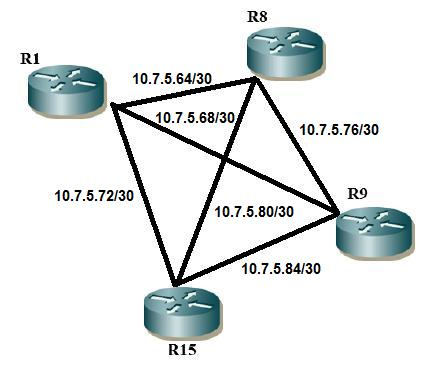
\includegraphics[width=0.8\textwidth]{Imagenes/framerelay1.jpg}
      	\end{center}
      	\captionof{figure}{Diagrama Frame Relay}
      	\label{figFr001}
			\end{figure}

			Para confeccionar la red Frame-Relay en el gns3 se utilizó el dispositivo \textit{FrameRelay-Switch}. El mismo permite configurar de forma amigable
			a través de un entorno GUI el enrutamiento de los paquetes que llegan al mismo a partir de los DLCIs. Con este dispositivo configurado, 
			sólo basta configurar las interfaces de los routers involucrados en la nube Frame-Relay para dejar operativa a la misma. \\
			\indent  Las interfaces que están conectadas a la red Frame-Relay deben ser interfaces Seriales (esto se debe a que los DTEs envían y reciben información
			a través del protocolo RS-232). Se debe especificar por la interfaz que salen los paquetes que los mismos deben ser encapsulados por medio de Frame-Relay. 
			Luego, como solo existe un enlace serial entre cada router y la nube, se implementan interfaces virtuales para cada uno de los enlaces punto a punto entre
			los routers. En cada uno de estos enlaces debe determinarse con que DLCI serán enviados los paquetes salientes de cada una de las interfaces. 
			A continuación, se exhibe la configuración pertinente a Frame-Relay implementada en cada uno de los routers conectados a la nube: \\

			\textbf{R1:}
			\begin{verbatim}
				interface Serial1/0
				no ip address
				encapsulation frame-relay
				
				interface Serial1/0.1 point-to-point
				ip address 10.7.5.65 255.255.255.252
				frame-relay interface-dlci 108

				interface Serial1/0.2 point-to-point
				ip address 10.7.5.69 255.255.255.252
				frame-relay interface-dlci 109

				interface Serial1/0.3 point-to-point
				ip address 10.7.5.73 255.255.255.252
				frame-relay interface-dlci 105
			\end{verbatim}	

			\vspace{0.5cm}
			\textbf{R8:}
			\begin{verbatim}
				interface Serial1/0
				no ip address
				encapsulation frame-relay

				interface Serial1/0.1 point-to-point
				ip address 10.7.5.66 255.255.255.252
				frame-relay interface-dlci 801

				interface Serial1/0.2 point-to-point
				ip address 10.7.5.77 255.255.255.252
				frame-relay interface-dlci 809

				interface Serial1/0.3 point-to-point
				ip address 10.7.5.81 255.255.255.252
				frame-relay interface-dlci 805
			\end{verbatim}	
			
			\vspace{0.5cm}
			\textbf{R9:}
			\begin{verbatim}
				interface Serial1/0
				no ip address
				encapsulation frame-relay

				interface Serial1/0.1 point-to-point
				ip address 10.7.5.70 255.255.255.252
				frame-relay interface-dlci 901

				interface Serial1/0.2 point-to-point
				ip address 10.7.5.78 255.255.255.252
				frame-relay interface-dlci 908

				interface Serial1/0.3 point-to-point
				ip address 10.7.5.85 255.255.255.252
				frame-relay interface-dlci 905
			\end{verbatim}	

			\vspace{0.5cm}
			\textbf{R15:}
			\begin{verbatim}
				interface Serial1/0
				no ip address
				encapsulation frame-relay

				interface Serial1/0.1 point-to-point
				ip address 10.7.5.74 255.255.255.252
				frame-relay interface-dlci 501

				interface Serial1/0.2 point-to-point
				ip address 10.7.5.82 255.255.255.252
				frame-relay interface-dlci 508

				interface Serial1/0.3 point-to-point
				ip address 10.7.5.86 255.255.255.252
				frame-relay interface-dlci 509
			\end{verbatim}
	

	\vspace{0.5cm}	
	\subsection{Tunnel GRE}
		\indent	Utilizando el tutorial expuesto en la cátedra, se creó un Tunnel GRE para encapsular en la red las conexiones de los routers R7 y R13 a Internet. 
		En la tabla \ref{tab002} se exhiben, entre otros, los datos de las subredes involucradas en el Tunnel. En la figura \ref{figGRE001} se exhibe 
		el equivalente de la topología luego de implementar el Tunnel. Gracias al mismo, se crea una conexión punto a punto entre R7 y R13, de forma que las 
		subredes \textit{Kentia} y \textit{Ulmaria} no son vistas en la red.
			\begin{figure}[!htbp]
    	  \centering
     	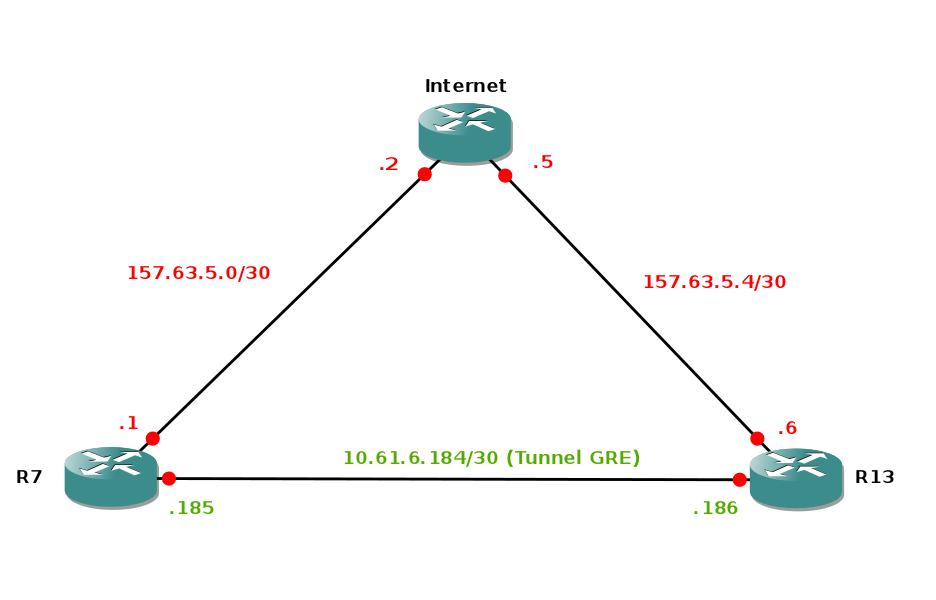
\includegraphics[width=12cm]{Imagenes/tunnelGRE.jpg}
     	 \captionof{figure}{Diagrama Tunnel GRE}
      	\label{figGRE001}
			\end{figure}

		Se exhibe a continuación, la configuración pertinente al protocolo GRE en los routers R7 y R13. Además de la configuración expuesta en el tutorial, se debe
		configurar de forma estática la comunicación de R7 a R13 y R13 a R7 a través de internet. De no especificarse esto, el Tunnel no se puede formar dado que 
		el protocolo no conoce como hacer para llegar desde un router, es decir, no saben que la comunicación entre R7 y R13 se realiza a través del router que
		simboliza Internet.  \\

		\textbf{R7:}
		\begin{verbatim}
			interface tunnel 10
			ip address 10.61.6.185 255.255.255.252
			tunnel source 157.63.5.1
			tunnel destination 157.63.5.6
			ip route 157.63.5.4 	255.255.255.252 	157.63.5.2
		\end{verbatim}

		\vspace{0.5cm}
		\textbf{R13:}
		\begin{verbatim}
			interface tunnel 20
			ip address 10.61.6.186 255.255.255.252
			tunnel source 157.63.5.6
			tunnel destination 157.63.5.1
			ip route 157.63.5.0 	255.255.255.252 	157.63.5.5
		\end{verbatim}	

	\vspace{0.5cm}	
	\subsection{VRRP - Virtual Router Redundancy Protocol}
		Vrrp es un protocolo de redundancia definido en el RFC 3768. El objetivo de vrrp es
		mantenter disponible una puerta de enlace para una determinada red. Para ello se
		define un router virtual y se configuran dos o más routers fisicos, de los cuales 
		solo uno va a realizar realmente el enrutamiento. Si el router fisíco falla o 
		alguna de sus interfaces (sobre las cuales se aplica el protocolo) cae, se negocia
		mediante el transpaso de mensajes quien es el próximo router que toma el rol de 
		maestro.\\
		En el caso del presente trabajo, se aplicó vrrp en dos pares de routers, por un 
		lado se aplicó a los routers R3 y R4, los cuales tienen en común la red A, y por
		el otro se aplicó a los routers R5 y R6 los cuales tienen interfaces en las redes 
		L y B.\\
		A continuación se muestra como se aplicó el protocolo en ambos casos.
		
		\subsubsection{Redundancia R3/R4}
			\textbf{R3:}
			En el caso de R3 se definió un tracking object que sensara la interface
			Ethernet0/2, correspondiente a la red A, y luego se configuró 
			dicha interface con los parametros de vrrp, se le asigno una prioridad de
			110, se definió la ip virtual 192.168.25.6. Por último se definió un 
			intervalo de 15 segundos para el intercambio de mensajes y un decremento 
			de 20 para la prioridad, según lo indique el tracking object.
			\begin{verbatim}
				hostname R3

				track 1 interface Ethernet0/2 ip routing

				interface Ethernet0/2
				ip address 192.168.25.4 255.255.255.0
				vrrp 12 description vrrp_lan_1
				vrrp 12 priority 110
				vrrp 12 timers advertise 15
				vrrp 12 timers learn
				vrrp 12 ip 192.168.25.6
				vrrp 12 track 1 decrement 20
			\end{verbatim}

			\textbf{R4:}
			En R4 no es necesario el tracking object, por lo que solo se configuraron
			los parametros correspondientes a vrrp mencionados anteriormente.
			\begin{verbatim}
				hostname R4

				interface ethernet0/2
				ip address 192.168.25.5 255.255.255.0
				vrrp 12 description vrrp_lan_3
				vrrp 12 priority 100
				vrrp 12 timers advertise 15
				vrrp 12 timers learn
				vrrp 12 ip 192.168.25.6
			\end{verbatim}

		\subsubsection{Redundancia R5/R6}
			\textbf{R5:}
			Tanto para R5 como para R6, se configuraron dos de las interfaces de los
			routers, puesto que son dos redes las que tienen en común (B y L). A la
			interface Ethernet0/0 correspondiente a la red L, se le configuró vrrp 10
			con ip virtual 10.61.6.196 y prioridad 100, mientras que a la interface 
			Ethernet0/1 correspondiente a la red B, se le configuro vrrp 11 con ip 
			virtual 10.111.25.196 y la misma prioridad.
			\begin{verbatim}
				hostname R5

				interface Ethernet0/0
				ip address 10.61.6.194 255.255.255.224
				vrrp 10 description vrrp_lan_1
				vrrp 10 priority 100
				vrrp 10 timers advertise 15
				vrrp 10 timers learn
				vrrp 10 ip 10.61.6.196

				interface Ethernet0/1
				ip address 10.111.25.194 255.255.255.192
				vrrp 11 description vrrp_lan_2
				vrrp 11 priority 100
				vrrp 11 timers advertise 15
				vrrp 11 timers learn
				vrrp 11 ip 10.111.25.196
			\end{verbatim}

			\textbf{R6:}
			Al igual que el caso anterior, en R6 se configuraron dos interfaces, y 
			ademas se definieron dos tracking objects qhe sensaran dichas interfaces. 
			Por un lado se definió el tracking object 1 sobre la interface Ethernet0/1
			en la cual se aplica vrrp 10, con ip virtual 10.61.6.196 como se mencionó
			anteriormente y prioridad 110. El segundo tracking object se aplicó sobre
			la interface Ethernet0/2 en la cual se definió vrrp 11, con ip virtual 
			10.111.25.196 y prioridad 110 (al igual que antes). La diferencia sustancial
			con la configuración de R3 y R4, es que en este caso, por mas que falle una
			de las dos inerfaces, se le decrementa la prioridad a ambas.
			\begin{verbatim}
				hostname R6

				track 1 interface Ethernet0/1 ip routing
				track 2 interface Ethernet0/2 ip routing

				interface Ethernet0/1
				ip address 10.61.6.195 255.255.255.224
				vrrp 10 description vrrp_lan_1
				vrrp 10 priority 110
				vrrp 10 timers advertise 15
				vrrp 10 timers learn
				vrrp 10 ip 10.61.6.196
				vrrp 10 track 1 decrement 20
				vrrp 10 track 2 decrement 20

				interface Ethernet0/2
				ip address 10.111.25.193 255.255.255.192
				vrrp 11 description vrrp_lan_2
				vrrp 11 priority 110
				vrrp 11 timers advertise 15
				vrrp 11 timers learn
				vrrp 11 ip 10.111.25.196
				vrrp 11 track 1 decrement 20
				vrrp 11 track 2 decrement 20
			\end{verbatim}
\newpage
\section{DNS}

Existen tres servidores DNS y tres zonas: 
\begin{itemize}	
	\item Mercedes 
	\item Zárate 
	\item	Azul
\end{itemize}

El DNS Root está en la red \textbf{Amapola} de la zona \textbf{Mercedes} con ip 192.168.25.7. Delega la autoridad en los restantes dos 
servidores de nivel dos, por lo que sólo tiene registros NS apuntando hacia los otros servidores DNS de nivel dos. La autoridad de los 
servidores de nivel dos se reparte de la siguiente manera (Ver Figura \ref{dns001}): \\

\begin{itemize}
 \item DNS1, en la red \textbf{Dalia} de la zona \textbf{Azul} con ip 10.111.25.131, para la zona AZUL
 \item DNS2, en la red \textbf{Bergonia} de la zona \textbf{Zárate} con ip 10.111.25.197, para el resto de las zonas
\end{itemize}

\begin{figure}[!htpb]
      \centering
      \begin{center}
      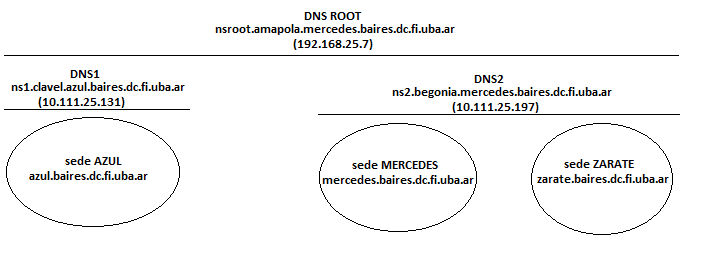
\includegraphics[width=11cm]{Imagenes/dns.png}
      \end{center}
      \caption{Esquema de delegación de dns}
      \label{dns001}
\end{figure}

\indent La parte más compleja de este servidor está en la delegación del mapeo reverso. Se adoptó la práctica común de crear nuevos 
nombres canónicos y hacer a la direcciones IP reales aliases de las primeras, en una relación uno a uno. En conjunto con la creación 
de una zona por cada subnet y la posterior delegación de autoridad sobre esta zona al servidor que se desea que tenga autoridad sobre 
las IPs reales, se logra el cometido. En caso de no estar subneteado, se procede similarmente, delegando cada dirección al nameserver 
correspondiente. Por simplificación se usó el statement \$GENERATE. \\

\indent Es decir, para el mapeo reverso, se creo una zona por cada subnet no alieneada a los objetos de la dirección ip (máscara /24). 
Dentro de esta zona, se delega cada host al servidor DNS de nivel dos correspondiente. El árbol de espacio de nombres de dominios 
(solo teniendo en cuenta los hosts especiales y sus respectivas direciones IPs) se puede apreciar en la Figura \ref{dns002}. \\

\begin{figure}[!htpb]
      \centering
      \begin{center}
      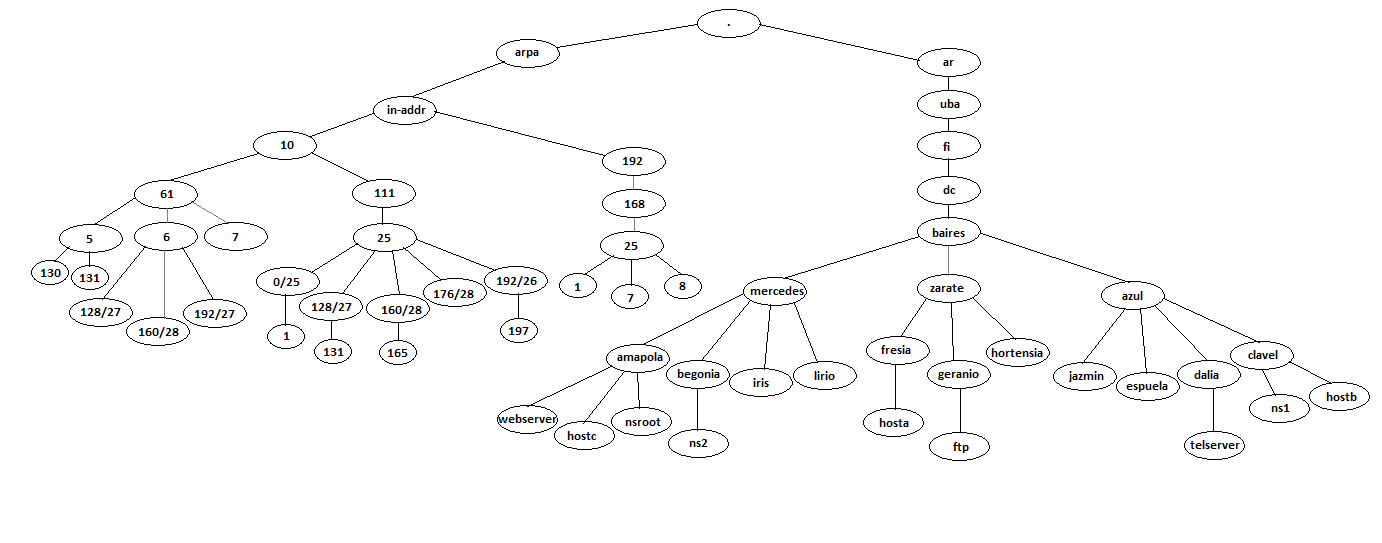
\includegraphics[width=20cm, angle=90]{Imagenes/dns2.png}
      \end{center}
      \caption{Árbol de espacio de nombres de dominio}
      \label{dns002}
\end{figure}


\indent Los host que corren los DNS de nivel tienen como servidor de espacio de nombres al Root, por lo que si se cae este último, los servidores de 
nivel dos serán incapaces de resolver querys incluso para zonas sobre las que tienen autoridad. \\ 

\begin{table}[!htbp]
	\centering
	\begin{tabular}{|c|c|c|c|}   
		\hline
		\multicolumn{4}{|c|}{\textbf{Mercedes}} \\
		\hline
		\hline
		\multicolumn{4}{|c|}{\textbf{Amapola - 192.168.25.0/24 - (.amapola.mercedes.baires.dc.fi.uba.ar)}} \\
		\hline
		Host & Dirección & Nombre & Dominio \\
		\hline
		WebServer & 192.168.25.1 & webserver & www.baires.dc.fi.uba.ar \\
		\hline 
		R1 & 192.168.25.2 & r1 & - \\
		\hline
		R2 & 192.168.25.3 & r2 & - \\
 		\hline
		R3 & 192.168.25.4 & r3 & - \\
		\hline
		R4 & 192.168.25.5 & r4 & - \\
		\hline
		\multirow{2}{*}{DNSRoot} & \multirow{2}{*}{192.168.25.7} & \multirow{2}{*}{nsroot} & ns.baires.dc.fi.uba.ar \\
			& & & nsroot.baires.dc.fi.uba.ar \\
		\hline
		\multirow{2}{*}{HostC} & \multirow{2}{*}{192.168.25.8} & \multirow{2}{*}{hostc} & hostc.baires.dc.fi.uba.ar \\
			& & & c.baires.dc.fi.uba.ar \\
		\hline
		\hline
		\multicolumn{4}{|c|}{\textbf{Begonia - 10.111.25.192/26 - (.begonia.mercedes.baires.dc.fi.uba.ar)}} \\
		\hline
		Host & Dirección & Nombre & Dominio \\
		\hline
		R6 & 10.111.25.193 & r6 & - \\
		\hline
		R18 & 10.111.25.194 & r7 & - \\
		\hline
		DNS2 & 10.111.25.195 & ns2 & ns2.baires.dc.fi.uba.ar \\
		\hline
		\hline
		\multicolumn{4}{|c|}{\textbf{Iris - 10.111.25.176/28 - (.iris.mercedes.baires.dc.fi.uba.ar)}} \\
		\hline
		Host & Dirección & Nombre & Dominio \\
		\hline
		R3 & 10.111.25.177 & r3 & - \\
		\hline
		R4 & 10.111.25.178 & r4 & - \\
		\hline
		\hline
		\multicolumn{4}{|c|}{\textbf{Lirio - 10.61.6.192/27 - (.lirio.mercedes.baires.dc.fi.uba.ar)}} \\
		\hline
		Host & Dirección & Nombre & Dominio \\
		\hline
		R4 & 10.61.6.193 & r4 & - \\
		\hline
		R5 & 10.61.6.194 & r5 & - \\
		\hline
		R6 & 10.61.6.195 & r6 & - \\
		\hline
 	\end{tabular}
	\caption{Esquema de asignaciones en Mercedes}
\end{table}

\begin{table}[!htbp]
	\centering
	\begin{tabular}{|c|c|c|c|}   
		\hline
		\multicolumn{4}{|c|}{\textbf{Azul}} \\
		\hline
		\hline
		\multicolumn{4}{|c|}{\textbf{Clavel - 10.61.5.0/24 - (.clavel.azul.baires.dc.fi.uba.ar)}} \\
		\hline
		Host & Dirección & Nombre & Dominio \\
		\hline
		R16 & 10.61.5.1 & r16 & - \\
		\hline 
		R17 & 10.61.5.2 & r17 & - \\
		\hline
		TelServer & 10.61.5.130 & telserver & telserver.baires.dc.fi.uba.ar \\
 		\hline
		\multirow{2}{*}{Host B} & \multirow{2}{*}{10.61.5.131} & \multirow{2}{*}{hostb} & hostb.baires.dc.fi.uba.ar \\
			& & & b.baires.dc.fi.uba.ar \\
		\hline
		\hline
		\multicolumn{4}{|c|}{\textbf{Dalia - 10.111.25.128/27 - (.dalia.azul.baires.dc.fi.uba.ar)}} \\
		\hline
		Host & Dirección & Nombre & Dominio \\
		\hline
		R17 & 10.111.25.129 & r17 & - \\
		\hline
		R18 & 10.111.25.130 & r18 & - \\
		\hline
		DNS1 & 10.111.25.131 & ns1 & ns1.baires.dc.fi.uba.ar \\
		\hline
		\hline
		\multicolumn{4}{|c|}{\textbf{Espuela - 10.61.6.128/27 - (.espuela.azul.baires.dc.fi.uba.ar)}} \\
		\hline
		Host & Dirección & Nombre & Dominio \\
		\hline
		R14 & 10.61.6.130 & r14 & - \\
		\hline
		R15 & 10.61.6.131 & r15 & - \\
		\hline
		R16 & 10.61.6.132 & r16 & - \\
		\hline
		\hline
		\multicolumn{4}{|c|}{\textbf{Jazmín - 10.61.6.160/28 - (.jazmin.azul.baires.dc.fi.uba.ar)}} \\
		\hline
		Host & Dirección & Nombre & Dominio \\
		\hline
		R18 & 10.61.6.161 & r18 & - \\
		\hline
 	\end{tabular}
	\caption{Esquema de asignaciones en Azul}
\end{table}

\begin{table}[!tbp]
	\centering
	\begin{tabular}{|c|c|c|c|}   
		\hline
		\multicolumn{4}{|c|}{\textbf{Zárate}} \\
		\hline
		\hline
		\multicolumn{4}{|c|}{\textbf{Fresia - 10.111.25.160/28 - (.fresia.zarate.baires.dc.fi.uba.ar)}} \\
		\hline
		Host & Dirección & Nombre & Dominio \\
		\hline
		R10 & 10.111.25.161 & r10 & - \\
		\hline 
		R17 & 10.111.25.162 & r11 & - \\
		\hline
		R12 & 10.111.25.162 & r12 & - \\
		\hline
		R13 & 10.111.25.163 & r13 & - \\
 		\hline
		\multirow{2}{*}{Host C} & \multirow{2}{*}{10.111.25.165} & \multirow{2}{*}{hosta} & hosta.baires.dc.fi.uba.ar \\
			& & & a.baires.dc.fi.uba.ar \\
		\hline
		\hline
		\multicolumn{4}{|c|}{\textbf{Geranio - 10.111.25.0/25 - (.geranio.zarate.dc.fi.uba.ar)}} \\
		\hline
		Host & Dirección & Nombre & Dominio \\
		\hline
		FTP Server & 10.111.25.1 & ftp & ftp.baires.dc.fi.uba.ar \\
		\hline
		R12 & 10.111.25.1 & r12 & - \\
		\hline
		\hline
		\multicolumn{4}{|c|}{\textbf{Hortensia - 10.61.7.128/25 - (.hortensia.zarate.baires.dc.fi.uba.ar)}} \\
		\hline
		Host & Dirección & Nombre & Dominio \\
		\hline
		R7 & 10.61.7.129 & r7 & - \\
		\hline
		R9 & 10.61.7.130 & r8 & - \\
		\hline
		R10 & 10.61.7.131 & r10 & - \\
		\hline
		R11 & 10.61.7.132 & r12 & - \\
		\hline
 	\end{tabular}
	\caption{Esquema de asignaciones en Zárate}
\end{table}

\newpage
\section{Servicios}
	\subsection{Webserver}

	\indent Hypertext Transfer Protocol o HTTP es el protocolo usado en cada transacción de la World Wide Web.  Es un protocolo orientado a transacciones y sigue el esquema petición-respuesta entre \textit{un cliente y un servidor}. Al cliente que efectúa la petición (en general un navegador web) se lo conoce como \textit{user agent}. A la información transmitida se la llama \textit{recurso} y se la identifica mediante un localizador uniforme de recursos (URL).
\indent El servidor HTTP Apache es un servidor web HTTP de código abierto, para plataformas Unix (BSD, GNU/Linux, etc.) y es el que se pretende emplear, particularmente en versión 2.
\indent Se requiere para el servidor web dos configuraciones:
\begin{itemize}
\item Ubicar en la carpeta /etc/apache2/ del servidor el archivo apache2.conf con la configuración estándar del servidor relacionada al ambiente global. Debido a que el enunciado no hace mención sobre la configuración del servidor web, se elige la configuración estándar de apache2.

\item Ubicar en la carpeta /var/www/ del servidor las páginas que se desean proveer a los clientes. Se ha desarrollado una página default, index.html.
\end{itemize}

\indent El puerto utilizado por default es el 8080 y se configura a través del archivo /etc/apache2/ports.conf.\\
\indent Será posible luego, para un cliente, acceder a algún recurso del servidor web, a través de una petición de consola, o a través de una request en un cliente web, solicitando al url:

\url{http://direccion_servidor:8080/index.html}
o simplemente
\url{http://direccion_servidor:8080/}


	\subsection{Telnet}
		\indent Telnet es un protocolo de red que permite la comunicación remota a otro host a través de una consola de comandos. Como FTP, es un
		protocolo orientado a la conexión que corre bajo TCP a través de una arquitectura \textit{Cliente-Servidor}. El puerto predeterminado de 
		\textit{telnet} es el 23. Debido a lo vulnerable que se vuelve el equipo que implementa este servicio, el mismo por lo general va acompañado
		por algún protocolo que provea de la seguridad necesaria como \textit{ssh}. \\
		\indent En el caso del presente trabajo práctico, debido a que el enunciado no hace mención sobre la configuración del servidor Telnet el, mismo no 
		realiza autenticación alguna del cliente que desea conectarse ni se encarga de encriptar la información que viaja entre el Cliente y el Servidor. \\
		\indent El servicio de Telnet a instalar es \textit{telnetd}. Luego de instalar el mismo, este se debe correr a través del service dispatcher
		\textit{inetd}. \textit{inetd} es un demonio que atiende las solicitudes de conexión que llegan al equipo, llamando al servicio que deba atender
		al llamado de conexión en función del puerto por el cual vino la misma. En el caso de \textit{telnet}, \textit{inetd} llamará a este servicio cada
		vez que llegue una solicitud de conexión a través del puerto 23. \\
		\indent Para verificar que el mismo levante las conexiones \textit{telnet} hay que asegurarse
		que en el archivo de configuración de \textit{inetd} (/etc/inetd.conf)  se encuentre la línea correspondiente a telnet y que la misma no se 
		encuentre comentada. La misma se exhibe a continuación: \\
		\begin{verbatim}
			telnet		stream	tcp	nowait	root	/usr/sbin/tcpd	/usr/sbin/in.telnetd
		\end{verbatim} 

	\subsection{FTP}
		\indent FTP es un protocolo de red utilizado para intercambiar archivos entre hosts. El mismo es un protocolo orientado a la conexión,	
		implementado bajo una arquitectura \textit{Cliente-Servidor}. El mismo corre bajo TCP y utiliza como número de puerto al realizar
		una conexión el 21. De entre los muchos servicios FTP existentes, se eligió utilizar el 
		servicio \textbf{vsftpd}. El mismo se puede descargar sin problemas de los repositorios de cualquier distribución de GNU/Linux. Como
		cualquier servicio, luego de instalarlo el mismo es levantado cada vez que el sistema operativo bootea. \\
		\indent El archivo de configuración de \textbf{vsftpd} se encuentra en el directorio \textit{/etc}. Debido a que el enunciado no 
		hace mención sobre la configuración del servidor FTP, se elige la misma de forma arbitraria. A continuación se muestra el contenido
		del archivo de configuración de vsftd.conf, obviando los comentarios de forma que queden visibles las líneas relevantes:	
		
		\begin{verbatim}
			listen=YES
			anonymous_enable=YES
			local_enable=YES
			write_enable=YES
			local_umask=022
			dirmessage_enable=YES
			use_localtime=YES
			xferlog_enable=YES
			connect_from_port_20=NO
			chroot_local_user=YES
			secure_chroot_dir=/var/run/vsftpd/empty
			pam_service_name=vsftpd
			rsa_cert_file=/etc/ssl/private/vsftpd.pem
		\end{verbatim}

		Muchas de los comandos aquí mostrados vienen por defecto al instalar el servicio. Sin embargo, se debe prestar atención a algunos es especial.
		Dado que el objetivo del TP es poder montar un servidor FTP y que los hosts conectados a la topología puedan interactuar con el mismo, se tienen
		en cuenta los siguientes puntos:
		\begin{itemize}
			\item Se desea que los clientes no se tengan que autenticar a la hora de realizar una conexión con el servidor. De esta forma, es necesario que
			en el archivo de configuración se encuentre la línea \textit{anonymous\_enable=YES}.
			\item Debido a que las pruebas del presente trabajo se van a realizar en un laboratorio, es necesario que el servidor FTP permita la conexión
			de host locales. Esto se especifica a partir de la línea \textit{local\_enable=YES}.
			\item Se desea que el cliente pueda subir archivos al servidor cuando el mismo lo desee. Para darle este beneficio, es necesario que en el 
			archivo de configuración se encuentre la línea \textit{write\_enable=YES}. 
			\item Se desea aprisonar (Chroot Jail) al cliente en el directorio en el cual se loguea el mismo. Esta decisión es totalmente arbitraria y simplemente
			fue colocada para probar algunas funcionalidades provistas por \textbf{vsftpd}. La principal funcionalidad de que un cliente se encuentre en una 
			\textit{Chroot Jail} consiste en que el mismo no pueda subir a directorios superiores al que le fue asignado y pueda alterar datos de otro usuario o de
			la máquina servidora en sí. De esta forma, para aprisonar al cliente en su carpeta de logueo se debe agregar al línea \textit{chroot\_local\_user=YES}.
		\end{itemize}

		Las líneas que no se mencionan que se encuentran en el archivo de configuración o bien no son lo suficientemente relevantes para ser explicadas, o bien
		no fueron investigadas o testeadas a fondo como para realmente saber la importancia de las mismas. Se dejan las mismas dado que el servidor funciona
		con las mismas. 


\newpage
\section{Tunnel VPN}

Puesto que los servicios (como el servidor Web, Telnet, FTP y DNS) asi como tambien una serie de 
host particulares (Host A, B y C) se deben correr en computadoras separadas a la que se simula 
la topología con GNS3, se debió buscar un mecanismo que permita comunicar todas las computadoras,
sin alterar a su vez la red global sobre la cual se realizan las simulaciones.\\
Dicho mecanismo fue el de implementar una serie de VPNs (Virtual Private Networks) entre la 
computadora sobre la cual se simula la topología y el resto de las terminales.\\
Una VPN es una tecnología de red que permite una extención segura de una red local, la cual se 
encuentra corriendo sobre una red global (en nuestro caso la red de la facultad). Se dice que es 
una extención segura puesto que una vpn debe garantizar:\\

\begin{itemize}
	\item Autentificación
	\item Integridad
	\item Confidencialidad
	\item No repudio
\end{itemize} 

Sin embargo, dado que en nuestro caso el objetivo de la vpn es no inundar la red global con
paquetes propios (por ejemplo paquetes ARP de la simulación), solo se utilizó la vpn 
como un mecanismo de tunneling y no se aplicó ningún método de encriptación.\\

Para la implementación de la vpn, se opto por usar OpenVPN, el cual es un daemon basado en 
OpenSSL, el cual soporta, seguridad SSL/TLS, ethernet bridging, tunneling TCP o UDP, entre
otros. Como se mencionó anteriormente, el objetivo principal de la vpn en nuestro caso es el de
generar un tunel que permita regular el tráfico que la topología envía a la red global.\\
Para simplificar el diseño, en la maquina donde se ejecuta la topología, se crearon 
dispositivos tap con números fijos para cada una de las terminales necesarias (WebServer, Host A, 
DNS1, etc). Una vez creados los tap, en la topología se colocó un dispositivo \textit{Cloud} que 
representase a cada terminal y se le asignó a cada uno el tap correspondiente. A continuación se 
muestra la tabla \ref{tab063} con la configuración resultante de el número de tap y el puerto 
por el cual se comunican las computadoras.

\begin{table}[!htbp]
	\centering
	\begin{tabular}{|c|c|c|c|}
	\hline
	Terminal & Dispositivo & Puerto \\	
	\hline
	DNS1 & tap1 & 1195 \\
	\hline
	DNS2 & tap2 & 1196 \\
	\hline
	DNS Root & tap3 & 1197 \\
	\hline
	FTP Server & tap4 & 1198 \\
	\hline
	Web Server & tap5 & 1199 \\
	\hline
	Telnet Server C & tap6 & 1200 \\
	\hline
	Telnet Server E & tap7 & 1201 \\
	\hline
	Host A & tap8 & 1202 \\
	\hline
	Host B & tap9 & 1203 \\
	\hline
	Host C & tap10 & 1204 \\
	\hline
	\end{tabular}
	\caption{Tabla de las VPNs}
	\label{tab063}
\end{table}

La configuración del lado de las terminales es mucho mas simple, puesto que solo es necesarió que
exista un único tap creado por vez, de acuerdo al servició o host que se este simulando en el 
momento. Para conectar dicha terminal con la topología solo basta crear un dispositivo tap al 
cual se le indica la dirección IP de la computadora corriendo la topología y el número de puerto 
al que se debe conectar, asi como tambien la dirección IP y mascara que dicho dispositivo debe
tener en la red simulada.


\newpage
\begin{thebibliography}{99}
	\bibitem{RFC} ``Internet Standard Subnetting Procedure'' RFC 950, 1985.  Mogul, J., Postel, J..
	\bibitem{RFC} ``Virtual Router Redundancy Protocol'' RFC 3768.  R. Hinden.
	\bibitem{WWW} ``DNS for Rocket Scientists''  \url{http://www.zytrax.com/books/dns}
	\bibitem{WWW} ``Linux Man page''
\end{thebibliography}
\end{document}


